\section{Campaign details}
\label{app:campaign}

This appendix lists the checkpoints and their consumed loci, the acceptance decisions, the coverage of the campaign, and the per-concept results of every completed block.

\subsection{Labels, registration, and artifact}
\label{app:cf-labels}

\paragraph{Labels.} We use the report-derived labels supplied with each dataset (NIH ChestX-ray14 finding labels; the CheXpert labeler output distributed with CheXpert Plus; COCO instance annotations). A row is positive for label 1, negative for label 0, and \emph{unknown} when the labeler output is uncertain or blank. We exclude unknown rows from probe fitting, selectivity, and answer AUROC. We write and score them like all other rows. Fixed manifests drawn with recorded seeds define the cohorts. Training and test cohorts are patient-disjoint. Every cohort is disjoint from every seed-study cohort. Table~\ref{tab:cf-prevalence} gives per-concept counts. A second CheXpert cohort contains \cfValidRows{} frontal films from the CheXpert validation set, one per patient, with the radiologists' consensus labels. It has zero patient overlap with any campaign cohort (Table~\ref{tab:cf-valid}).

\paragraph{Registration.} We froze the protocol before scoring any grid block. The loci, projection and probe settings, dose, reference family, six templates, module set, seven gates, and three decision rules match the registered protocol file and its code commit. We registered the seed study's crossover and confirmation analyses before running them (Appendix~\ref{app:seed}). One analysis pass over the packaged outcomes produces everything reported per block. After completing the grid, we added the leaderboard, write-flow share, and per-image examples as descriptive summaries of these outputs.

\paragraph{Artifact.} The release includes evaluation code and adapters, the registered protocol file, cohort manifests with their seeds, fitted directions, per-image outcomes for every module (write, dose, refit, locus, and template rows), scorecards and coverage files for every block, and rendered prompts. Adding a new checkpoint requires one adapter that identifies the block it consumes and passes the gates.

\subsection{Grid and consumed loci}
\label{app:cf-grid}

\begin{table}[h]
\centering
\scriptsize
\setlength{\tabcolsep}{3pt}
\caption{\textbf{Checkpoint sheet.} Family, parameters, vision tower, consumed visual tokens per image at the primary locus, input image size, eligible question templates after the image-free mapping gate (I/W: ``is''/``show'' wording; Y: yes/no; A/B: letter mappings), completed dataset blocks, and GPU-hours of scoring (A100-80GB).}
\label{tab:cf-models}
\resizebox{\textwidth}{!}{%
\begin{tabular}{llrllllr}
\toprule
Checkpoint & Family & Params & Vision tower & Tokens & Image & Templates & Blocks (GPU-h) \\
\midrule
Qwen2.5-VL-3B & Qwen2.5-VL & 3B & native ViT 675M & 576$\to$144 & $336^2$ & IYWYIAWA & NIH (13), CXP (3), COCO (13) \\
Qwen2.5-VL-7B & Qwen2.5-VL & 7B & native ViT 675M & 576$\to$144 & $336^2$ & all & NIH (27), CXP (5), COCO (26) \\
Qwen2.5-VL-32B & Qwen2.5-VL & 32B & native ViT 675M & 576$\to$144 & $336^2$ & all & NIH (83), CXP (16), COCO (75) \\
Qwen2.5-VL-72B & Qwen2.5-VL & 72B & native ViT 675M & 576$\to$144 & $336^2$ & all & NIH (214) \\
Qwen3-VL-4B & Qwen3-VL & 4B & SigLIP2-based & $\leq$1024 & $\leq 512^2$ & all & NIH (15), CXP (3), COCO (14) \\
Qwen3-VL-8B & Qwen3-VL & 8B & SigLIP2-based & $\leq$1024 & $\leq 512^2$ & all & NIH (26), CXP (5), COCO (20) \\
Qwen3-VL-32B & Qwen3-VL & 32B & SigLIP2-based & $\leq$1024 & $\leq 512^2$ & all & NIH (106), CXP (28), COCO (98) \\
InternVL3.5-8B & InternVL3.5 & 8B & InternViT-300M & 1024 & $448^2$ & all & NIH (19), CXP (4), COCO (18) \\
InternVL3.5-14B & InternVL3.5 & 14B & InternViT-300M & 1024 & $448^2$ & all & NIH (29), CXP (5), COCO (28) \\
Gemma 3 4B & Gemma 3 & 4B & SigLIP-So400m & 4096 & $896^2$ & all & NIH (22), CXP (9), COCO (34) \\
Gemma 3 12B & Gemma 3 & 12B & SigLIP-So400m & 4096 & $896^2$ & all & NIH (40), CXP (11), COCO (52) \\
Gemma 3 27B & Gemma 3 & 27B & SigLIP-So400m & 4096 & $896^2$ & all & NIH (129), CXP (29), COCO (119) \\
MedGemma 4B & MedGemma & 4B & MedSigLIP & 4096 & $896^2$ & all & NIH (44), CXP (9), COCO (36) \\
MedGemma 27B & MedGemma & 27B & MedSigLIP & 4096 & $896^2$ & all & NIH (118), CXP (33), COCO (74) \\
Lingshu 7B & Lingshu & 7B & Qwen2.5-VL ViT & 576$\to$144 & $336^2$ & all & NIH (20), CXP (5), COCO (20) \\
Lingshu 32B & Lingshu & 32B & Qwen2.5-VL ViT & 576$\to$144 & $336^2$ & all & NIH (74), CXP (19), COCO (76) \\
LLaVA-1.5-7B & LLaVA-1.5 & 7B & CLIP ViT-L/14-336 & 576 & $336^2$ & IYWY & NIH (21), CXP (7), COCO (20) \\
LLaVA-1.5-13B & LLaVA-1.5 & 13B & CLIP ViT-L/14-336 & 576 & $336^2$ & IYWYIAWA & NIH (34), CXP (10), COCO (38) \\
LLaVA-Med 1.5 7B & LLaVA-Med & 7B & CLIP ViT-L/14-336 & 576 & $336^2$ & IYWY & NIH (20), CXP (7), COCO (22) \\
Llama 3.2 Vision 11B & Llama 3.2 Vision & 11B & ViT-H/14 & 1601 & $560^2$ & IBWB & NIH (22), CXP (0), COCO (22) \\
\bottomrule
\end{tabular}}
\end{table}

\begin{table}[h]
\centering
\scriptsize
\setlength{\tabcolsep}{4pt}
\caption{\textbf{Preflight gates.} Each block is scored only after the seven checks below run on 16 held-out rows at both loci; the right column gives the range observed over all completed blocks.}
\label{tab:cf-gates}
\begin{tabular}{clp{4.3cm}p{6.0cm}}
\toprule
Gate & Name & Criterion & Observed \\
\midrule
A & Determinism & identical answer logits on a repeated forward & max difference 0 \\
B & Identity at $\alpha=0$ & the armed hook with zero dose changes nothing & max difference 0 \\
C & Reach & the write changes the consumer input and the answer logits; no change outside consumed tokens & consumer change 0.44--29.84; answer logits 0.20--23.82; outside consumed tokens 0 \\
D & Batch consistency & single- vs batched-forward answer logits within 0.25 & 0.07--1.84; above tolerance (declared, neutralised by fixed batch composition): Qwen2.5-VL ($\leq$0.37), Qwen3-VL ($\leq$1.41), InternVL3.5 ($\leq$0.62), Gemma 3 ($\leq$1.84), MedGemma ($\leq$0.56), Lingshu ($\leq$0.30), LLaVA-1.5 ($\leq$0.31), Llama 3.2 Vision ($\leq$0.41) \\
E & Semantic mapping & image-free ``present/absent'' statements map to the right answer token under each template & failing templates: LLaVA-1.5-13B: IBWB; LLaVA-1.5-7B: IAIBWAWB; LLaVA-Med 1.5 7B: IAIBWAWB; Llama 3.2 Vision 11B: IYWYIAWA; Qwen2.5-VL-3B: IBWB \\
F & Throughput & rows per second recorded for scheduling & 3.8--35 rows/s \\
G & fp32 answer logits & fp32 logits recomputed from the final hidden state agree with the model's bf16 logits & max difference 0.12 \\
\bottomrule
\end{tabular}
\end{table}

\begin{table}[t]
\centering
\scriptsize
\setlength{\tabcolsep}{3pt}
% Morandi tints for the cf-transfer tables (muted, low saturation); darker = larger value
\definecolor{cfSage1}{HTML}{EEF1EA}
\definecolor{cfSage2}{HTML}{D9E1D2}
\definecolor{cfSage3}{HTML}{C1CDB8}
\definecolor{cfSage4}{HTML}{A6B79C}
\definecolor{cfSlate1}{HTML}{ECEFF2}
\definecolor{cfSlate2}{HTML}{D3DAE2}
\definecolor{cfSlate3}{HTML}{B7C3D0}
\definecolor{cfSlate4}{HTML}{98A8B9}
\definecolor{cfTerra1}{HTML}{F5ECE9}
\definecolor{cfTerra2}{HTML}{E9D3CC}
\definecolor{cfTerra3}{HTML}{DAB5AA}
\definecolor{cfTerra4}{HTML}{C9968A}
\definecolor{cfOat1}{HTML}{F4EFE6}
\definecolor{cfOat2}{HTML}{E8DDC8}
\definecolor{cfGrey}{HTML}{E4E1DC}

\caption{\textbf{Families.} Vision tower, sizes evaluated, medical fine-tuning, consumed visual tokens per image at the primary locus, mean probe selectivity and clean-answer AUROC over clinical cells, owned clinical and COCO cells, and the mean of three controls over blocks: signed dose range of $O_q$ (DOSE module), refit SD over three seeds, and $|$connector-locus median $O_q|$. Owned counts are shaded slate (darker = larger share).}
\label{tab:cf-families}
\resizebox{\textwidth}{!}{%
\begin{tabular}{llllrrrrrrrr}
\toprule
Family & Vision tower & Sizes & Med. & Tokens & $\bar S$ & $\overline{\mathrm{AUROC}}$ & Owned clin. & Owned COCO & Dose & Refit SD & $|O_\mathrm{conn}|$ \\
\midrule
Qwen2.5-VL & native ViT 675M & 3B/7B/32B/72B & no & 576$\to$144 & 0.122 & 0.625 & \cellcolor{cfSlate2}4/42 & \cellcolor{cfSlate4}18/18 & +0.46 & 0.076 & 0.014 \\
Qwen3-VL & SigLIP2-based & 4B/8B/32B & no & $\leq$1024 & 0.137 & 0.735 & \cellcolor{cfSlate2}4/36 & \cellcolor{cfSlate4}18/18 & +0.50 & 0.042 & 0.006 \\
InternVL3.5 & InternViT-300M / InternViT-6B & 8B/14B/38B & no & 1024 & 0.125 & 0.807 & \cellcolor{cfSlate2}5/36 & \cellcolor{cfSlate4}17/18 & +0.04 & 0.004 & 0.004 \\
Gemma 3 & SigLIP-So400m & 4B/12B/27B & no & 4096 & 0.124 & 0.564 & \cellcolor{cfSlate2}2/36 & \cellcolor{cfSlate4}17/18 & +0.57 & 0.102 & 0.023 \\
MedGemma & MedSigLIP & 4B/27B & yes & 4096 & 0.164 & 0.835 & \cellcolor{cfSlate2}2/24 & \cellcolor{cfSlate3}10/12 & +0.39 & 0.068 & 0.006 \\
Lingshu & Qwen2.5-VL ViT & 7B/32B & yes & 576$\to$144 & 0.142 & 0.820 & \cellcolor{cfSlate4}11/24 & \cellcolor{cfSlate4}12/12 & +0.38 & 0.047 & 0.008 \\
LLaVA-1.5 & CLIP ViT-L/14-336 & 7B/13B & no & 576 & 0.124 & 0.516 & \cellcolor{cfSlate1}0/24 & \cellcolor{cfSlate3}7/12 & +0.06 & 0.010 & 0.021 \\
LLaVA-Med & CLIP ViT-L/14-336 & 7B & yes & 576 & 0.136 & 0.560 & \cellcolor{cfSlate2}1/12 & \cellcolor{cfSlate2}1/6 & +0.03 & 0.008 & 0.012 \\
Llama 3.2 Vision & ViT-H/14 & 11B & no & 1601 & 0.119 & 0.688 & \cellcolor{cfSlate1}0/12 & \cellcolor{cfSlate2}1/6 & +0.08 & 0.035 & 0.039 \\
\bottomrule
\end{tabular}}
\end{table}

\begin{figure}[h]
    \centering
    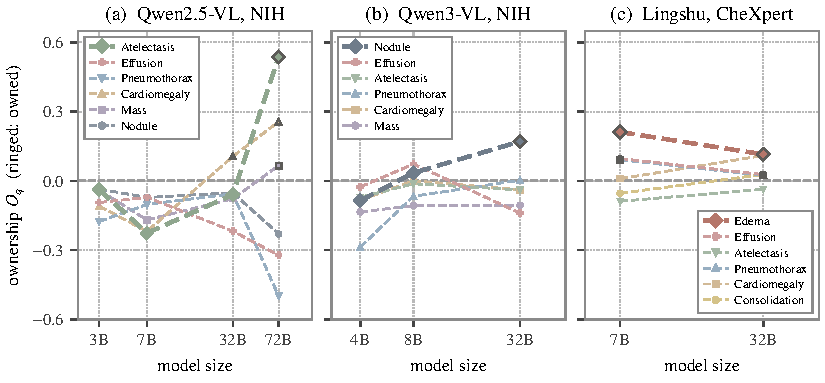
\includegraphics[width=\textwidth]{figures/fig6_ladders.pdf}
    \caption{\textbf{Size ladders.} Ownership $O_q$ per concept across sizes for Qwen2.5-VL on NIH, Qwen3-VL on NIH, and Lingshu on CheXpert. The concept with the largest ownership at the largest size is drawn bold (Atelectasis, Nodule, Edema); ringed markers are owned cells.}
    \label{fig:ladders}
\end{figure}

\begin{table}[h]
\centering
\scriptsize
\setlength{\tabcolsep}{4pt}
\caption{\textbf{Label counts per concept.} Positive / negative / unknown rows in the training and test cohorts of the fixed manifests (unknown = CheXpert labeler uncertain or blank; unknown rows are excluded from probe fitting, selectivity, and answer AUROC, and scored like every other row under every write).}
\label{tab:cf-prevalence}
\begin{tabular}{llrrrrrr}
\toprule
Dataset & Concept & \multicolumn{3}{c}{train (pos / neg / unk)} & \multicolumn{3}{c}{test (pos / neg / unk)} \\
\midrule
NIH ChestX-ray14 & Effusion & 2423 & 15789 & 0 & 46 & 554 & 0 \\
 & Atelectasis & 2311 & 15901 & 0 & 57 & 543 & 0 \\
 & Pneumothorax & 1254 & 16958 & 0 & 17 & 583 & 0 \\
 & Cardiomegaly & 881 & 17331 & 0 & 23 & 577 & 0 \\
 & Mass & 1263 & 16949 & 0 & 32 & 568 & 0 \\
 & Nodule & 1549 & 16663 & 0 & 47 & 553 & 0 \\
\addlinespace
CheXpert Plus & Effusion & 5897 & 4277 & 9826 & 158 & 130 & 312 \\
 & Atelectasis & 2891 & 86 & 17023 & 84 & 2 & 514 \\
 & Pneumothorax & 1086 & 6456 & 12458 & 32 & 213 & 355 \\
 & Cardiomegaly & 2312 & 1903 & 15785 & 71 & 58 & 471 \\
 & Consolidation & 966 & 3652 & 15382 & 25 & 113 & 462 \\
 & Edema & 3814 & 2231 & 13955 & 133 & 59 & 408 \\
\addlinespace
COCO & person & 10877 & 9123 & 0 & 321 & 279 & 0 \\
 & dog & 693 & 19307 & 0 & 15 & 585 & 0 \\
 & car & 2051 & 17949 & 0 & 60 & 540 & 0 \\
 & chair & 2183 & 17817 & 0 & 63 & 537 & 0 \\
 & bottle & 1455 & 18545 & 0 & 47 & 553 & 0 \\
 & bicycle & 567 & 19433 & 0 & 14 & 586 & 0 \\
\bottomrule
\end{tabular}
\end{table}


For Llama~3.2 Vision, the projector also reads five intermediate local-layer outputs that bypass the final global block. LLaVA computes the final CLIP block but consumes the penultimate block instead. For every checkpoint, Gate (C) verifies that the write reaches the consumer and the answer logits while changing nothing outside the consumed tokens.

\subsection{Acceptance decisions}
\label{app:cf-gates}

All \cfWriteBlocks{} completed blocks pass checks (A), (B), (C), and (G) with zero determinism error, zero change at $\alpha=0$, and fp32-versus-model logit differences below \cfGateFpMax{}. In check (D), the Qwen3-VL, Gemma~3, MedGemma, InternVL, and Llama families exceed the 0.25-logit tolerance (up to \cfGateBatchMax{} logits for Gemma~3 12B). We record these as declared deviations. Fixed batch composition neutralises them. Check (E) fails on all datasets for the A/B templates for LLaVA-1.5-7B and LLaVA-Med, the B-mapped templates for Qwen2.5-VL-3B and LLaVA-1.5-13B, and the yes/no and A-mapped templates for Llama~3.2 Vision 11B. We record the affected cells as ineligible. Two checkpoints answer ``yes'' to nearly every chest question (Gemma~3 4B: clean $P(\mathrm{yes})>0.99$ on \cfGemmaFourYesMin--\cfGemmaFourYesMax\% of rows). The answerability grade records this behaviour. Three checkpoints (LLaVA-1.5 7B/13B, LLaVA-Med) answer at chance.

\subsection{Coverage and cost}
\label{app:cf-coverage}

\cfCheckpointsCompleteWord{} checkpoints are complete on all three datasets (Table~\ref{tab:cf-coverage}). Coverage includes all modules on NIH and COCO---the write matrix, calibration, the five additional templates, the dose sweep, the two refits, and the connector locus---and the write matrix and calibration on CheXpert. We grade Llama~3.2 Vision 11B on its eligible B-positive template IB. Qwen2.5-VL-72B is complete on NIH. The compute budget prevented runs of the 72B COCO/CheXpert blocks and Llama~3.2 Vision 90B. InternVL3.5-38B is complete on all three datasets. The campaign used about 3,000 A100-hours. A chest block for a 7B checkpoint takes about ten GPU-hours.

\begin{table}[h]
\centering
\scriptsize
\setlength{\tabcolsep}{4pt}
\caption{\textbf{Coverage.} Modules completed per block at packaging (from the campaign manifest), with the modules whose template is ineligible (inel.) and the primary template when it is not the \emph{is}/yes-no template; ``--'' = block not run; modules still in progress are not listed. \cfCoverageBlocksAllSeven{} blocks carry all seven modules of the planned campaign, and the five modules added to CheXpert after the first wave are complete on \cfCoverageChexFull{} of the CheXpert blocks.}
\label{tab:cf-coverage}
\begin{tabular}{llll}
\toprule
Checkpoint & NIH ChestX-ray14 & CheXpert Plus & COCO \\
\midrule
Qwen2.5-VL-3B & C Cal P D R L Lc A Ad & C Cal A Ad & C Cal P D R L Lc A Ad \\
Qwen2.5-VL-7B & C Cal P D R L Lc A Ad An E T Pr & C Cal P D R L Lc A Ad An E T & C Cal P D R L Lc A Ad An T Pr \\
Qwen2.5-VL-32B & C Cal P D R L Lc A Ad & C Cal P D R L Lc A Ad & C Cal P D R L Lc A Ad \\
Qwen2.5-VL-72B & C Cal P D R L Lc & -- & -- \\
Qwen3-VL-4B & C Cal P D R L Lc A Ad & C Cal A Ad & C Cal P D R L Lc A Ad \\
Qwen3-VL-8B & C Cal P D R L Lc A Ad E T & C Cal A Ad & C Cal P D R L Lc A Ad T \\
Qwen3-VL-32B & C Cal P D R L Lc A Ad & C Cal D R Lc A Ad & C Cal P D R L Lc A Ad \\
InternVL3.5-8B & C Cal P D R L Lc A Ad E & C Cal A Ad & C Cal P D R L Lc A Ad \\
InternVL3.5-14B & C Cal P D R L Lc A Ad & C Cal A Ad & C Cal P D R L Lc A Ad \\
InternVL3.5-38B & C Cal P D R L Lc A & C Cal A & C Cal P D R L Lc A \\
Gemma 3 4B & C Cal P D R L Lc A Ad & C Cal A Ad & C Cal P D R L Lc A Ad \\
Gemma 3 12B & C Cal P D R L Lc A Ad An E T & C Cal A Ad An E & C Cal P D R L Lc A Ad An \\
Gemma 3 27B & C Cal P D R L Lc & C Cal A & C Cal P D R L Lc A \\
MedGemma 4B & C Cal P D R L Lc A Ad & C Cal A Ad E & C Cal P D R L Lc A Ad \\
MedGemma 27B & C Cal P D R L Lc A Ad & C Cal A & C Cal P D R L Lc A \\
Lingshu 7B & C Cal P D R L Lc A Ad & C Cal D R Lc A Ad & C Cal P D R L Lc A Ad \\
Lingshu 32B & C Cal P D R L Lc A Ad An E & C Cal A Ad An E & C Cal P D R L Lc A Ad An \\
LLaVA-1.5-7B & C Cal P D R L Lc A Ad & C Cal P D R L Lc A Ad & C Cal P D R L Lc A Ad \\
LLaVA-1.5-13B & C Cal P D R L Lc A Ad & C Cal A Ad & C Cal P D R L Lc A Ad \\
LLaVA-Med 1.5 7B & C Cal P D R L Lc A Ad & C Cal A Ad & C Cal P D R L Lc A Ad \\
Llama 3.2 Vision 11B & C Cal P D R L Lc A [IB] & C Cal D R L Lc A [IB] & C Cal P D R L Lc A [IB] \\
\midrule
\multicolumn{4}{p{0.95\textwidth}}{\textit{Legend:} C = CORE, Cal = CALIBRATION, P = PROMPT, D = DOSE, R = REFIT, L = LOCUS, Lc = LOCUS\_CALIBRATION, A = ALTDIR, Ad = ALTDIRD, An = ANSDIR, E = EXTCOMP, T = TOKENW, Pr = PRECISION.} \\
\bottomrule
\end{tabular}
\end{table}


\subsection{Ownership of every concept}
\label{app:cf-tables}

Tables~\ref{tab:cf-own-nih}--\ref{tab:cf-own-coco} report the ownership contrast for every concept cell. Figure~\ref{fig:cf-w-structure} summarises the structure of the underlying write matrices. Figure~\ref{fig:cf-examples} shows grades for individual images.

\begin{table}[h]
\centering
\scriptsize
\setlength{\tabcolsep}{4pt}
\renewcommand{\arraystretch}{1.08}
% Morandi tints for the cf-transfer tables (muted, low saturation); darker = larger value
\definecolor{cfSage1}{HTML}{EEF1EA}
\definecolor{cfSage2}{HTML}{D9E1D2}
\definecolor{cfSage3}{HTML}{C1CDB8}
\definecolor{cfSage4}{HTML}{A6B79C}
\definecolor{cfSlate1}{HTML}{ECEFF2}
\definecolor{cfSlate2}{HTML}{D3DAE2}
\definecolor{cfSlate3}{HTML}{B7C3D0}
\definecolor{cfSlate4}{HTML}{98A8B9}
\definecolor{cfTerra1}{HTML}{F5ECE9}
\definecolor{cfTerra2}{HTML}{E9D3CC}
\definecolor{cfTerra3}{HTML}{DAB5AA}
\definecolor{cfTerra4}{HTML}{C9968A}
\definecolor{cfOat1}{HTML}{F4EFE6}
\definecolor{cfOat2}{HTML}{E8DDC8}
\definecolor{cfGrey}{HTML}{E4E1DC}

\caption{\textbf{Ownership on NIH ChestX-ray14.} Each cell is the ownership contrast $O_q$ of the concept's own write against its strongest clinical competitor at $\alpha=+0.25$. Cells are shaded slate for positive and terracotta for negative values (darker = larger magnitude, thresholds $0.02$, $0.10$, $0.25$). Bold marks owned cells (steering reference met and all simultaneous lower bounds $>0$). A dagger marks cells whose write meets the steering reference but loses to a competitor. Grey ``inel.'' marks checkpoints whose yes/no template is ineligible. Checkpoints are in the order of Table~\ref{tab:cf-main}.}
\label{tab:cf-own-nih}
\begin{tabular}{lrrrrrr}
\toprule
Checkpoint & Effusion & Atelectasis & Pneumothorax & Cardiomegaly & Mass & Nodule \\
\midrule
Lingshu 32B & \cellcolor{cfTerra1}-0.01 & \cellcolor{cfTerra2}-0.08 & \cellcolor{cfSlate3}\textbf{+0.14} & \cellcolor{cfSlate2}\textbf{+0.05} & \cellcolor{cfTerra2}-0.08 & \cellcolor{cfTerra3}-0.18 \\
Qwen2.5-VL-72B & \cellcolor{cfTerra4}-0.32 & \cellcolor{cfSlate4}\textbf{+0.54} & \cellcolor{cfTerra4}-0.50 & \cellcolor{cfSlate4}\textbf{+0.26} & \cellcolor{cfSlate2}\textbf{+0.07} & \cellcolor{cfTerra3}-0.23 \\
Lingshu 7B & \cellcolor{cfSlate1}+0.02 & \cellcolor{cfSlate1}+0.01 & \cellcolor{cfSlate1}+0.01 & \cellcolor{cfSlate3}\textbf{+0.17} & \cellcolor{cfTerra2}-0.09 & \cellcolor{cfSlate1}+0.02 \\
Qwen3-VL-4B & \cellcolor{cfTerra2}-0.03$^{\dagger}$ & \cellcolor{cfTerra2}-0.07 & \cellcolor{cfTerra4}-0.29 & \cellcolor{cfTerra2}-0.08 & \cellcolor{cfTerra3}-0.13 & \cellcolor{cfTerra2}-0.09 \\
Qwen3-VL-32B & \cellcolor{cfTerra3}-0.14 & \cellcolor{cfTerra2}-0.04 & \cellcolor{cfSlate1}+0.00$^{\dagger}$ & \cellcolor{cfTerra2}-0.04 & \cellcolor{cfTerra3}-0.11 & \cellcolor{cfSlate3}\textbf{+0.17} \\
Gemma 3 12B & \cellcolor{cfTerra4}-0.83 & \cellcolor{cfTerra4}-0.57 & \cellcolor{cfTerra3}-0.17 & \cellcolor{cfTerra3}-0.19 & \cellcolor{cfTerra4}-0.65 & \cellcolor{cfSlate3}\textbf{+0.17} \\
MedGemma 4B & \cellcolor{cfSlate1}+0.01 & \cellcolor{cfTerra4}-0.56 & \cellcolor{cfSlate1}+0.01 & \cellcolor{cfTerra2}-0.07 & \cellcolor{cfTerra4}-0.27 & \cellcolor{cfSlate2}+0.09 \\
InternVL3.5-14B & \cellcolor{cfSlate1}\textbf{+0.01} & \cellcolor{cfTerra1}-0.01 & \cellcolor{cfTerra1}-0.00 & \cellcolor{cfTerra1}-0.00 & \cellcolor{cfSlate1}+0.00 & \cellcolor{cfTerra1}-0.01 \\
Qwen2.5-VL-32B & \cellcolor{cfTerra3}-0.22 & \cellcolor{cfTerra2}-0.06 & \cellcolor{cfTerra2}-0.06 & \cellcolor{cfSlate3}\textbf{+0.11} & \cellcolor{cfTerra2}-0.08 & \cellcolor{cfTerra2}-0.05 \\
InternVL3.5-8B & \cellcolor{cfSlate1}+0.00 & \cellcolor{cfTerra1}-0.02 & \cellcolor{cfTerra1}-0.00 & \cellcolor{cfSlate1}+0.00 & \cellcolor{cfTerra1}-0.01 & \cellcolor{cfTerra1}-0.01 \\
LLaVA-Med 1.5 7B & \cellcolor{cfTerra1}-0.00 & \cellcolor{cfTerra1}-0.00 & \cellcolor{cfTerra2}-0.04 & \cellcolor{cfTerra1}-0.01 & \cellcolor{cfTerra1}-0.01 & \cellcolor{cfTerra2}-0.02 \\
Qwen2.5-VL-3B & \cellcolor{cfTerra2}-0.09 & \cellcolor{cfTerra2}-0.04 & \cellcolor{cfTerra3}-0.18 & \cellcolor{cfTerra3}-0.11 & \cellcolor{cfTerra2}-0.04 & \cellcolor{cfTerra2}-0.04 \\
Qwen2.5-VL-7B & \cellcolor{cfTerra2}-0.07$^{\dagger}$ & \cellcolor{cfTerra3}-0.23 & \cellcolor{cfTerra3}-0.10 & \cellcolor{cfTerra3}-0.22 & \cellcolor{cfTerra3}-0.17 & \cellcolor{cfTerra2}-0.07 \\
Qwen3-VL-8B & \cellcolor{cfSlate2}+0.07 & \cellcolor{cfTerra1}-0.01 & \cellcolor{cfTerra2}-0.07 & \cellcolor{cfSlate1}+0.00 & \cellcolor{cfTerra3}-0.11 & \cellcolor{cfSlate2}+0.03 \\
InternVL3.5-38B & \cellcolor{cfSlate1}+0.00$^{\dagger}$ & \cellcolor{cfTerra1}-0.02 & \cellcolor{cfTerra1}-0.00 & \cellcolor{cfTerra2}-0.03 & \cellcolor{cfSlate1}+0.02 & \cellcolor{cfSlate1}+0.00 \\
Gemma 3 27B & \cellcolor{cfTerra2}-0.04 & \cellcolor{cfTerra2}-0.03 & \cellcolor{cfTerra1}-0.01 & \cellcolor{cfSlate1}+0.00$^{\dagger}$ & \cellcolor{cfTerra2}-0.08 & \cellcolor{cfTerra1}-0.02 \\
Gemma 3 4B & \cellcolor{cfTerra1}-0.00 & \cellcolor{cfTerra1}-0.00 & \cellcolor{cfTerra1}-0.01 & \cellcolor{cfTerra3}-0.24 & \cellcolor{cfTerra4}-0.28 & \cellcolor{cfTerra3}-0.12 \\
LLaVA-1.5-7B & \cellcolor{cfTerra2}-0.03 & \cellcolor{cfTerra1}-0.01 & \cellcolor{cfTerra2}-0.08 & \cellcolor{cfTerra3}-0.13 & \cellcolor{cfSlate2}+0.02 & \cellcolor{cfTerra1}-0.02 \\
MedGemma 27B & \cellcolor{cfTerra2}-0.06 & \cellcolor{cfTerra4}-0.45 & \cellcolor{cfTerra1}-0.01 & \cellcolor{cfSlate1}+0.00 & \cellcolor{cfTerra3}-0.13 & \cellcolor{cfTerra3}-0.20 \\
LLaVA-1.5-13B & \cellcolor{cfTerra1}-0.01 & \cellcolor{cfTerra2}-0.05 & \cellcolor{cfTerra2}-0.04 & \cellcolor{cfTerra2}-0.03 & \cellcolor{cfSlate1}+0.01 & \cellcolor{cfTerra1}-0.02 \\
Llama 3.2 Vision 11B & \cellcolor{cfTerra2}-0.04 & \cellcolor{cfTerra2}-0.07 & \cellcolor{cfTerra2}-0.05 & \cellcolor{cfSlate2}+0.02 & \cellcolor{cfTerra2}-0.06 & \cellcolor{cfTerra1}-0.01 \\
\midrule
\textbf{Owned} & 1 & 1 & 1 & 4 & 1 & 2 \\
\bottomrule
\end{tabular}
\end{table}

\begin{table}[h]
\centering
\scriptsize
\setlength{\tabcolsep}{4pt}
\renewcommand{\arraystretch}{1.08}
% Morandi tints for the cf-transfer tables (muted, low saturation); darker = larger value
\definecolor{cfSage1}{HTML}{EEF1EA}
\definecolor{cfSage2}{HTML}{D9E1D2}
\definecolor{cfSage3}{HTML}{C1CDB8}
\definecolor{cfSage4}{HTML}{A6B79C}
\definecolor{cfSlate1}{HTML}{ECEFF2}
\definecolor{cfSlate2}{HTML}{D3DAE2}
\definecolor{cfSlate3}{HTML}{B7C3D0}
\definecolor{cfSlate4}{HTML}{98A8B9}
\definecolor{cfTerra1}{HTML}{F5ECE9}
\definecolor{cfTerra2}{HTML}{E9D3CC}
\definecolor{cfTerra3}{HTML}{DAB5AA}
\definecolor{cfTerra4}{HTML}{C9968A}
\definecolor{cfOat1}{HTML}{F4EFE6}
\definecolor{cfOat2}{HTML}{E8DDC8}
\definecolor{cfGrey}{HTML}{E4E1DC}

\caption{\textbf{Ownership on CheXpert Plus.} Each cell is the ownership contrast $O_q$ of the concept's own write against its strongest clinical competitor at $\alpha=+0.25$. Cells are shaded slate for positive and terracotta for negative values (darker = larger magnitude, thresholds $0.02$, $0.10$, $0.25$). Bold marks owned cells (steering reference met and all simultaneous lower bounds $>0$). A dagger marks cells whose write meets the steering reference but has a stronger competitor; a double dagger marks reference-meeting cells whose comparison is unresolved. Grey ``inel.'' marks checkpoints whose yes/no template is ineligible and grey ``inc.'' a write matrix incomplete at packaging (neither enters any count). Checkpoints are in the order of Table~\ref{tab:cf-main}.}
\label{tab:cf-own-chexpert}
\begin{tabular}{lrrrrrr}
\toprule
Checkpoint & Effusion & Atelectasis & Pneumothorax & Cardiomegaly & Consolidation & Edema \\
\midrule
Lingshu 32B & \cellcolor{cfSlate2}\textbf{+0.03} & \cellcolor{cfTerra2}-0.04$^{\dagger}$ & \cellcolor{cfSlate2}\textbf{+0.02} & \cellcolor{cfSlate3}\textbf{+0.11} & \cellcolor{cfSlate2}\textbf{+0.03} & \cellcolor{cfSlate3}\textbf{+0.11} \\
Lingshu 7B & \cellcolor{cfSlate2}\textbf{+0.10} & \cellcolor{cfTerra2}-0.09 & \cellcolor{cfSlate2}\textbf{+0.09} & \cellcolor{cfSlate1}+0.01$^{\ddagger}$ & \cellcolor{cfTerra2}-0.05 & \cellcolor{cfSlate3}\textbf{+0.21} \\
Qwen3-VL-4B & \cellcolor{cfTerra1}-0.01$^{\dagger}$ & \cellcolor{cfTerra1}-0.02 & \cellcolor{cfTerra3}-0.23 & \cellcolor{cfTerra1}-0.01 & \cellcolor{cfSlate2}\textbf{+0.09} & \cellcolor{cfSlate2}\textbf{+0.09} \\
Qwen3-VL-32B & \cellcolor{cfTerra2}-0.04 & \cellcolor{cfSlate1}+0.00$^{\ddagger}$ & \cellcolor{cfSlate1}+0.00 & \cellcolor{cfTerra2}-0.03 & \cellcolor{cfTerra3}-0.12 & \cellcolor{cfSlate2}\textbf{+0.05} \\
InternVL3.5-38B & \cellcolor{cfSlate1}\textbf{+0.02} & \cellcolor{cfTerra1}-0.01 & \cellcolor{cfTerra1}-0.00 & \cellcolor{cfTerra1}-0.00$^{\ddagger}$ & \cellcolor{cfSlate1}\textbf{+0.01} & \cellcolor{cfTerra2}-0.02 \\
Gemma 3 12B & \cellcolor{cfTerra4}-0.83 & \cellcolor{cfTerra3}-0.13 & \cellcolor{cfTerra4}-0.71 & \cellcolor{cfTerra4}-0.47 & \cellcolor{cfTerra4}-0.26 & \cellcolor{cfSlate3}\textbf{+0.15} \\
MedGemma 4B & \cellcolor{cfTerra3}-0.20 & \cellcolor{cfTerra2}-0.08 & \cellcolor{cfTerra4}-0.60 & \cellcolor{cfSlate2}\textbf{+0.04} & \cellcolor{cfTerra3}-0.20 & \cellcolor{cfSlate3}\textbf{+0.10} \\
InternVL3.5-14B & \cellcolor{cfSlate1}\textbf{+0.01} & \cellcolor{cfTerra1}-0.00 & \cellcolor{cfSlate1}+0.00 & \cellcolor{cfTerra1}-0.01 & \cellcolor{cfSlate1}+0.01 & \cellcolor{cfTerra1}-0.00 \\
Qwen2.5-VL-32B & \cellcolor{cfTerra2}-0.07 & \cellcolor{cfTerra3}-0.19 & \cellcolor{cfTerra3}-0.12 & \cellcolor{cfTerra3}-0.19 & \cellcolor{cfTerra2}-0.05 & \cellcolor{cfTerra2}-0.02 \\
InternVL3.5-8B & \cellcolor{cfTerra1}-0.01 & \cellcolor{cfTerra1}-0.01 & \cellcolor{cfSlate1}\textbf{+0.00} & \cellcolor{cfTerra1}-0.00 & \cellcolor{cfSlate1}+0.01 & \cellcolor{cfTerra1}-0.00 \\
LLaVA-Med 1.5 7B & \cellcolor{cfSlate1}\textbf{+0.00} & \cellcolor{cfTerra1}-0.00 & \cellcolor{cfTerra2}-0.02 & \cellcolor{cfTerra2}-0.03 & \cellcolor{cfTerra1}-0.00$^{\dagger}$ & \cellcolor{cfTerra1}-0.02 \\
Qwen2.5-VL-3B & \cellcolor{cfTerra3}-0.18 & \cellcolor{cfTerra1}-0.02 & \cellcolor{cfTerra2}-0.04 & \cellcolor{cfTerra2}-0.05 & \cellcolor{cfTerra2}-0.03 & \cellcolor{cfTerra2}-0.08 \\
Qwen2.5-VL-7B & \cellcolor{cfSlate1}+0.01 & \cellcolor{cfTerra2}-0.05 & \cellcolor{cfTerra2}-0.10 & \cellcolor{cfTerra1}-0.00 & \cellcolor{cfTerra3}-0.15 & \cellcolor{cfTerra3}-0.18 \\
Qwen3-VL-8B & \cellcolor{cfTerra2}-0.07$^{\dagger}$ & \cellcolor{cfTerra1}-0.00$^{\dagger}$ & \cellcolor{cfTerra2}-0.10 & \cellcolor{cfTerra1}-0.00 & \cellcolor{cfTerra2}-0.04$^{\dagger}$ & \cellcolor{cfTerra2}-0.06 \\
Gemma 3 27B & \cellcolor{cfTerra2}-0.03 & \cellcolor{cfTerra1}-0.00 & \cellcolor{cfTerra1}-0.01 & \cellcolor{cfTerra1}-0.00 & \cellcolor{cfTerra2}-0.03 & \cellcolor{cfSlate1}+0.00$^{\ddagger}$ \\
Gemma 3 4B & \cellcolor{cfTerra1}-0.00 & \cellcolor{cfTerra1}-0.00 & \cellcolor{cfTerra4}-0.65 & \cellcolor{cfTerra1}-0.02 & \cellcolor{cfTerra4}-0.35 & \cellcolor{cfTerra4}-0.58 \\
LLaVA-1.5-7B & \cellcolor{cfSlate1}+0.00 & \cellcolor{cfTerra2}-0.09 & \cellcolor{cfTerra2}-0.10 & \cellcolor{cfSlate2}+0.03 & \cellcolor{cfTerra2}-0.03 & \cellcolor{cfTerra1}-0.00 \\
MedGemma 27B & \cellcolor{cfTerra1}-0.01 & \cellcolor{cfSlate1}+0.00 & \cellcolor{cfTerra2}-0.06 & \cellcolor{cfSlate2}+0.03 & \cellcolor{cfTerra1}-0.02 & \cellcolor{cfTerra4}-0.28 \\
LLaVA-1.5-13B & \cellcolor{cfTerra1}-0.00 & \cellcolor{cfTerra2}-0.03 & \cellcolor{cfTerra1}-0.01 & \cellcolor{cfSlate1}+0.00 & \cellcolor{cfSlate1}+0.01 & \cellcolor{cfTerra1}-0.01 \\
Llama 3.2 Vision 11B & \cellcolor{cfGrey}inel. & \cellcolor{cfGrey}inel. & \cellcolor{cfGrey}inel. & \cellcolor{cfGrey}inel. & \cellcolor{cfGrey}inel. & \cellcolor{cfGrey}inel. \\
\midrule
\textbf{Owned} & 5 & 0 & 3 & 2 & 3 & 6 \\
\bottomrule
\end{tabular}
\end{table}

\begin{table}[h]
\centering
\scriptsize
\setlength{\tabcolsep}{4pt}
\renewcommand{\arraystretch}{1.08}
% Morandi tints for the cf-transfer tables (muted, low saturation); darker = larger value
\definecolor{cfSage1}{HTML}{EEF1EA}
\definecolor{cfSage2}{HTML}{D9E1D2}
\definecolor{cfSage3}{HTML}{C1CDB8}
\definecolor{cfSage4}{HTML}{A6B79C}
\definecolor{cfSlate1}{HTML}{ECEFF2}
\definecolor{cfSlate2}{HTML}{D3DAE2}
\definecolor{cfSlate3}{HTML}{B7C3D0}
\definecolor{cfSlate4}{HTML}{98A8B9}
\definecolor{cfTerra1}{HTML}{F5ECE9}
\definecolor{cfTerra2}{HTML}{E9D3CC}
\definecolor{cfTerra3}{HTML}{DAB5AA}
\definecolor{cfTerra4}{HTML}{C9968A}
\definecolor{cfOat1}{HTML}{F4EFE6}
\definecolor{cfOat2}{HTML}{E8DDC8}
\definecolor{cfGrey}{HTML}{E4E1DC}

\caption{\textbf{Ownership on COCO.} Each cell is the ownership contrast $O_q$ of the concept's own write against its strongest clinical competitor at $\alpha=+0.25$. Cells are shaded slate for positive and terracotta for negative values (darker = larger magnitude, thresholds $0.02$, $0.10$, $0.25$). Bold marks owned cells (steering reference met and all simultaneous lower bounds $>0$). A dagger marks cells whose write meets the steering reference but loses to a competitor. Grey ``inel.'' marks checkpoints whose yes/no template is ineligible. Checkpoints are in the order of Table~\ref{tab:cf-main}.}
\label{tab:cf-own-coco}
\begin{tabular}{lrrrrrr}
\toprule
Checkpoint & person & dog & car & chair & bottle & bicycle \\
\midrule
Lingshu 32B & \cellcolor{cfSlate4}\textbf{+0.29} & \cellcolor{cfSlate3}\textbf{+0.23} & \cellcolor{cfSlate2}\textbf{+0.08} & \cellcolor{cfSlate4}\textbf{+0.53} & \cellcolor{cfSlate4}\textbf{+0.34} & \cellcolor{cfSlate3}\textbf{+0.22} \\
Lingshu 7B & \cellcolor{cfSlate4}\textbf{+0.39} & \cellcolor{cfSlate4}\textbf{+0.74} & \cellcolor{cfSlate4}\textbf{+0.70} & \cellcolor{cfSlate4}\textbf{+0.76} & \cellcolor{cfSlate4}\textbf{+0.64} & \cellcolor{cfSlate4}\textbf{+0.85} \\
Qwen3-VL-4B & \cellcolor{cfSlate4}\textbf{+0.46} & \cellcolor{cfSlate3}\textbf{+0.13} & \cellcolor{cfSlate4}\textbf{+0.33} & \cellcolor{cfSlate4}\textbf{+0.71} & \cellcolor{cfSlate4}\textbf{+0.34} & \cellcolor{cfSlate2}\textbf{+0.07} \\
Qwen3-VL-32B & \cellcolor{cfSlate3}\textbf{+0.13} & \cellcolor{cfSlate3}\textbf{+0.12} & \cellcolor{cfSlate3}\textbf{+0.11} & \cellcolor{cfSlate3}\textbf{+0.23} & \cellcolor{cfSlate3}\textbf{+0.24} & \cellcolor{cfSlate2}\textbf{+0.07} \\
InternVL3.5-38B & \cellcolor{cfSlate1}\textbf{+0.01} & \cellcolor{cfSlate1}\textbf{+0.00} & \cellcolor{cfSlate1}\textbf{+0.01} & \cellcolor{cfSlate1}\textbf{+0.02} & \cellcolor{cfSlate1}\textbf{+0.01} & \cellcolor{cfSlate1}\textbf{+0.01} \\
Gemma 3 12B & \cellcolor{cfSlate3}\textbf{+0.19} & \cellcolor{cfSlate4}\textbf{+0.76} & \cellcolor{cfSlate4}\textbf{+0.48} & \cellcolor{cfSlate4}\textbf{+0.45} & \cellcolor{cfSlate3}\textbf{+0.18} & \cellcolor{cfSlate4}\textbf{+0.61} \\
MedGemma 4B & \cellcolor{cfSlate4}\textbf{+0.35} & \cellcolor{cfSlate2}\textbf{+0.03} & \cellcolor{cfSlate4}\textbf{+0.43} & \cellcolor{cfSlate3}\textbf{+0.19} & \cellcolor{cfSlate3}\textbf{+0.20} & \cellcolor{cfSlate3}\textbf{+0.14} \\
InternVL3.5-14B & \cellcolor{cfSlate1}\textbf{+0.02} & \cellcolor{cfSlate1}\textbf{+0.01} & \cellcolor{cfSlate1}\textbf{+0.01} & \cellcolor{cfSlate2}\textbf{+0.04} & \cellcolor{cfSlate2}\textbf{+0.03} & \cellcolor{cfSlate1}+0.00$^{\dagger}$ \\
Qwen2.5-VL-32B & \cellcolor{cfSlate4}\textbf{+0.44} & \cellcolor{cfSlate3}\textbf{+0.12} & \cellcolor{cfSlate4}\textbf{+0.27} & \cellcolor{cfSlate4}\textbf{+0.83} & \cellcolor{cfSlate4}\textbf{+0.41} & \cellcolor{cfSlate3}\textbf{+0.19} \\
InternVL3.5-8B & \cellcolor{cfSlate2}\textbf{+0.03} & \cellcolor{cfSlate1}\textbf{+0.01} & \cellcolor{cfSlate2}\textbf{+0.04} & \cellcolor{cfSlate2}\textbf{+0.04} & \cellcolor{cfSlate2}\textbf{+0.04} & \cellcolor{cfSlate1}\textbf{+0.02} \\
LLaVA-Med 1.5 7B & \cellcolor{cfSlate1}+0.02 & \cellcolor{cfSlate1}\textbf{+0.01} & \cellcolor{cfSlate1}+0.01 & \cellcolor{cfTerra2}-0.02 & \cellcolor{cfSlate1}+0.00 & \cellcolor{cfTerra1}-0.01 \\
Qwen2.5-VL-3B & \cellcolor{cfSlate4}\textbf{+0.46} & \cellcolor{cfSlate4}\textbf{+0.42} & \cellcolor{cfSlate4}\textbf{+0.53} & \cellcolor{cfSlate4}\textbf{+0.68} & \cellcolor{cfSlate4}\textbf{+0.61} & \cellcolor{cfSlate4}\textbf{+0.39} \\
Qwen2.5-VL-7B & \cellcolor{cfSlate4}\textbf{+0.48} & \cellcolor{cfSlate4}\textbf{+0.75} & \cellcolor{cfSlate4}\textbf{+0.61} & \cellcolor{cfSlate4}\textbf{+0.87} & \cellcolor{cfSlate4}\textbf{+0.51} & \cellcolor{cfSlate4}\textbf{+0.81} \\
Qwen3-VL-8B & \cellcolor{cfSlate4}\textbf{+0.42} & \cellcolor{cfSlate4}\textbf{+0.51} & \cellcolor{cfSlate4}\textbf{+0.74} & \cellcolor{cfSlate4}\textbf{+0.79} & \cellcolor{cfSlate4}\textbf{+0.59} & \cellcolor{cfSlate4}\textbf{+0.43} \\
Gemma 3 27B & \cellcolor{cfSlate3}\textbf{+0.24} & \cellcolor{cfSlate4}\textbf{+0.36} & \cellcolor{cfSlate2}\textbf{+0.09} & \cellcolor{cfSlate4}\textbf{+0.28} & \cellcolor{cfSlate3}\textbf{+0.15} & \cellcolor{cfSlate4}\textbf{+0.75} \\
Gemma 3 4B & \cellcolor{cfSlate3}\textbf{+0.16} & \cellcolor{cfSlate4}\textbf{+0.54} & \cellcolor{cfSlate3}\textbf{+0.24} & \cellcolor{cfSlate4}\textbf{+0.34} & \cellcolor{cfSlate4}\textbf{+0.44} & \cellcolor{cfTerra4}-0.27 \\
LLaVA-1.5-7B & \cellcolor{cfSlate2}\textbf{+0.06} & \cellcolor{cfSlate1}\textbf{+0.00} & \cellcolor{cfSlate1}\textbf{+0.01} & \cellcolor{cfSlate2}\textbf{+0.07} & \cellcolor{cfSlate1}+0.01 & \cellcolor{cfSlate1}\textbf{+0.00} \\
MedGemma 27B & \cellcolor{cfSlate4}\textbf{+0.33} & \cellcolor{cfTerra2}-0.04 & \cellcolor{cfSlate2}\textbf{+0.08} & \cellcolor{cfSlate3}\textbf{+0.18} & \cellcolor{cfSlate3}\textbf{+0.21} & \cellcolor{cfTerra2}-0.04 \\
LLaVA-1.5-13B & \cellcolor{cfSlate2}\textbf{+0.05} & \cellcolor{cfSlate1}+0.00$^{\dagger}$ & \cellcolor{cfSlate1}+0.02 & \cellcolor{cfSlate2}\textbf{+0.08} & \cellcolor{cfSlate1}+0.02 & \cellcolor{cfTerra2}-0.03 \\
Llama 3.2 Vision 11B & \cellcolor{cfGrey}inel. & \cellcolor{cfGrey}inel. & \cellcolor{cfGrey}inel. & \cellcolor{cfGrey}inel. & \cellcolor{cfGrey}inel. & \cellcolor{cfGrey}inel. \\
\midrule
\textbf{Owned} & 18 & 17 & 17 & 18 & 16 & 14 \\
\bottomrule
\end{tabular}
\end{table}

\begin{table}[t]
\centering
\small
\setlength{\tabcolsep}{4pt}
\caption{\textbf{Steering reference against verdict.} Primary write-matrix cells of the included blocks, cross-classified by the steering reference and by the simultaneous-bound verdict against the five other clinical directions.}
\label{tab:cf-contingency}
\begin{tabular}{llrrrr}
\toprule
Cells & Steering reference & advantage & stronger competitor & unresolved & total \\
\midrule
Chest, all cells & met & 29 & 8 & 7 & 44 \\
 & not met & 19 & 155 & 28 & 202 \\
Chest, readable and answerable & met & 21 & 4 & 3 & 28 \\
 & not met & 9 & 52 & 12 & 73 \\
COCO, all cells & met & 101 & 0 & 2 & 103 \\
 & not met & 6 & 10 & 1 & 17 \\
\bottomrule
\end{tabular}
\end{table}

\FloatBarrier

\subsection{Controls}
\label{app:cf-controls-sec}

Table~\ref{tab:cf-controls} summarises the reference family and the per-block controls of Section~\ref{sec:controls} across the grid.

\begin{table}[h]
\centering
\scriptsize
\setlength{\tabcolsep}{4pt}
\caption{\textbf{Reference family and controls.} Median and interquartile range over all cells (first four rows) or over all blocks with the corresponding module (next six rows), per dataset. The last three rows count the concept cells whose write meets the steering reference (above the random p95 and the sham), the owned cells, and the reference-meeting cells that miss the complete owned grade: their simultaneous advantage over the five clinical competitors is not positive. Table~\ref{tab:cf-contingency} splits these cells into stronger-competitor and unresolved cells.}
\label{tab:cf-controls}
\begin{tabular}{lrrrrrr}
\toprule
& \multicolumn{2}{c}{NIH ChestX-ray14} & \multicolumn{2}{c}{CheXpert Plus} & \multicolumn{2}{c}{COCO (control)} \\
\cmidrule(lr){2-3}\cmidrule(lr){4-5}\cmidrule(lr){6-7}
Quantity & median & IQR & median & IQR & median & IQR \\
\midrule
Random-family p95 of $W$ & +0.090 & [+0.034, +0.190] & +0.088 & [+0.027, +0.178] & +0.022 & [+0.009, +0.056] \\
$|$Sham write$|$ & +0.037 & [+0.013, +0.090] & +0.031 & [+0.010, +0.090] & +0.010 & [+0.003, +0.033] \\
Concept write $W_{qq}$ & +0.011 & [-0.011, +0.092] & +0.021 & [-0.000, +0.116] & +0.238 & [+0.035, +0.513] \\
Ownership $O_q$ & -0.028 & [-0.088, +0.001] & -0.014 & [-0.066, +0.001] & +0.178 & [+0.016, +0.442] \\
Signed dose range of $O_q$ & +0.266 & [+0.061, +0.444] & +0.162 & [+0.034, +0.359] & +0.399 & [+0.050, +0.612] \\
Refit SD of $O_q$ (3 seeds) & +0.039 & [+0.015, +0.072] & +0.037 & [+0.017, +0.052] & +0.043 & [+0.006, +0.074] \\
Connector-locus median $O_q$ & -0.013 & [-0.023, -0.005] & -0.009 & [-0.020, -0.004] & +0.003 & [+0.001, +0.007] \\
Label gap (logits) & -0.1 & [-0.9, -0.0] & -0.3 & [-1.3, +0.0] & -5.3 & [-14.8, -0.3] \\
$|$Wording contrast$|$ (IY$-$WY) & +0.033 & [+0.008, +0.078] & +0.021 & [+0.007, +0.035] & +0.028 & [+0.007, +0.065] \\
$|$Mapping contrast$|$ (IA$-$IB) & +0.037 & [+0.008, +0.073] & +0.019 & [+0.003, +0.055] & +0.030 & [+0.007, +0.051] \\
\midrule
Reference met & \multicolumn{2}{c}{15 of 126} & \multicolumn{2}{c}{29 of 120} & \multicolumn{2}{c}{103 of 120} \\
Owned & \multicolumn{2}{c}{10 of 126} & \multicolumn{2}{c}{19 of 120} & \multicolumn{2}{c}{101 of 120} \\
Reference met but not owned & \multicolumn{2}{c}{5 of 126} & \multicolumn{2}{c}{10 of 120} & \multicolumn{2}{c}{2 of 120} \\
\bottomrule
\end{tabular}
\end{table}



\subsection{Robustness of the deficit}
\label{app:cf-robustness}

The projected features are $x=R^{\top}\hvec$, where $R\in\R^{D\times512}$ is the fixed Gaussian projection. Two transformations map vectors from the projected, train-scaled space back to the consumed space. A classifier coefficient $\boldsymbol\beta$ lifts as $\hat\wvec\propto R\,\mathrm{diag}(1/\boldsymbol s)\boldsymbol\beta$, so the written direction scores the concept as the probe does (Equation~\ref{eq:lift}). A displacement $\boldsymbol u$ in that space lifts through its minimum-norm preimage as $\hat\wvec\propto R(R^{\top}R)^{-1}\mathrm{diag}(\boldsymbol s)\boldsymbol u$. This reproduces the displacement exactly: $R^{\top}\hat\wvec\propto\mathrm{diag}(\boldsymbol s)\boldsymbol u$. The lifts differ because $R^{\top}R$ is not a multiple of the identity. Measurements on every ALTDIRD block show that $R^{\top}R/D$ is full rank, with eigenvalues $\cfAltdirdEigMin$--$\cfAltdirdEigMax$ and condition number \cfAltdirdCondMin{}--\cfAltdirdCondMax{}. We compute the difference-of-means and pattern vectors in the projected space and report both lifts. The coefficient lift is the family the ALTDIR module scores (Table~\ref{tab:cf-altdir}). The displacement lift is the geometrically matched comparison for those two families (Table~\ref{tab:cf-altdird}): a difference of class means and a Haufe pattern are displacements in the projected space rather than classifier coefficients. The token-weighted variants multiply the per-token dose $\alpha\lVert\hvec_{it}\rVert$ by a weight $w_t$ with mean one over the consumed tokens. The softmax variant preserves the L1 dose of the uniform write. The top-quarter variant ($w_t=4$ on the 25\% highest-scoring tokens) has twice the uniform write's Frobenius norm. The attribute directions use three labels from each dataset's own metadata: the view field (anteroposterior or portable against posteroanterior), the recorded sex, and age at least 60. We fit these directions using the same images, features, projection, and probe settings as the clinical probes. We then lift and write them with the six clinical directions as one nine-direction family. Attribute questions have no random family, so the sham is their sole steering reference. Their probes reach a median AUROC of \cfAttrAurocMin{}--\cfAttrAurocMax{} against the attribute label and \cfAttrAnswerAurocMin{}--\cfAttrAnswerAurocMax{} against the model's own clean answer. The largest median $|\cos|$ between an attribute direction and a clinical normal is \cfAttrCosMax{}. Across the \cfAttrBlocks{} blocks with the module, the attributes are owned in \cfAttrChestAttrOwned{} of \cfAttrChestAttrN{} cells and the findings in the same family in \cfAttrChestClinOwned{} of \cfAttrChestClinN{}. The corresponding counts are \cfAttrChexAttrOwned{}/\cfAttrChexAttrN{} against \cfAttrChexClinOwned{}/\cfAttrChexClinN{} on CheXpert and \cfAttrNihAttrOwned{}/\cfAttrNihAttrN{} against \cfAttrNihClinOwned{}/\cfAttrNihClinN{} on NIH.

\paragraph{Direction and label geometry.} Neither correlations among the six directions nor co-occurrence of the six report labels explains why a competing direction wins (Table~\ref{tab:cf-geometry}). On NIH, the six directions are as orthogonal as random vectors (mean off-diagonal cosine $\cfGeoCosNih$ against $\cfGeoCosRandom$ for random pairs). The labels are nearly uncorrelated (mean $\phi=\cfGeoPhiNih$). Yet NIH shows the same off-diagonal dominance as CheXpert, where directions and labels are correlated (mean cosine $\cfGeoCosChex$; Effusion--Consolidation $\cfGeoCosEffCons$, $\phi=\cfGeoPhiEffCons$). The ownership contrast is positive, $O_q>0$, in \cfGeoOwnWinsNihPct\% of the \cfNihCells{} NIH cells and \cfGeoOwnWinsChexPct\% of the \cfChexCells{} CheXpert cells. The strongest competitor matches the most similar direction at chance rate (\cfGeoChanceCosMin{}--\cfGeoChanceCosMax\%) and the most co-occurring label at chance rate (\cfGeoChanceLabelMin{}--\cfGeoChanceLabelMax\%). Across the \cfGeoOffdiagCells{} off-diagonal chest cells, the competitor's advantage $W_{q,d}-W_{q,q}$ is uncorrelated with direction cosine (Spearman $\cfGeoRhoAdvCos$, $p=\cfGeoRhoAdvCosP$) and label $\phi$ ($\cfGeoRhoAdvPhi$). At least two competitors exceed the own write in \cfGeoTwoAbove{} of \cfGeoTwoAboveN{} chest cells (\cfGeoTwoAbovePct\%), so removing the strongest leaves $O_q$ negative in those cells. The $O_q^{-d^*}>0$ column of Table~\ref{tab:cf-geometry} counts the sign of $O_q$ after that removal, not the owned grade. The natural-image families with the highest co-occurrence (person with bicycle, $\phi=\cfGeoFamPhiPersonBicycle$; person with dog; chair with bottle) retain $O_q>0$ in \cfGeoCocoFamMinPct{}--\cfGeoCocoFamMaxPct\% of cells when competitors are restricted to those families. Of the five directions in the seed cell, Nodule is the \emph{least} similar to Effusion (cosine $\cfSeedCosNodule$). It still moves the Effusion answer more than Effusion's own direction ($\cfSeedWNodule$ against $\cfSeedWEff$). The most similar direction, Atelectasis (cosine $\cfSeedCosAtel$), moves it by $\cfSeedWAtel$.

\paragraph{Scale, saturation, refits, and numerics.} The grades hold on the logit scale. Recomputing the grade from the margin $\ell_{\mathrm{yes}}-\ell_{\mathrm{no}}$ reproduces the probability-scale owned grade in \cfScaleAgree{} of \cfScaleAgreeN{} cells. Every owned cell preserves the sign of its ownership contrast on that scale, $O^m_q>0$. The complete owned grade persists in \cfScaleOwnedKeepFull{} of the \cfScaleOwned{} owned cells, with the steering reference recomputed on the margin scale and a positive percentile interval for $O^m_q$ (Table~\ref{tab:cf-scale}). Saturation counters a ceiling explanation: COCO blocks have far more rows at $P(\mathrm{yes})>0.99$ or $<0.01$ than chest blocks (median block share $\cfScaleSatCoco$ against $\cfScaleSatNih$ and $\cfScaleSatChex$). Restricting each cell to its unsaturated rows preserves $O_q>0$ in all \cfScaleUnsatOwned{} owned chest cells and in \cfScaleUnsatOtherPos{} of the \cfScaleUnsatOther{} others. Full regrading of those rows, with the steering reference recomputed on them and the simultaneous max-$T$ advantage over the same six-direction family, preserves the owned grade in \cfScaleUnsatGradeKept{} of \cfScaleUnsatGradeN{} owned chest cells and raises \cfScaleUnsatGradeGained{} of the \cfScaleUnsatGradeOtherN{} others to owned. The same pattern holds in the clean-No, clean-Yes, label-present, and label-absent strata. Refitting the probes on resampled training patients changes $O_q$ by a median of $\cfScaleRefitMedian$. The bf16 batch effects declared at the gates (candidate-logit differences of $\cfScaleBatchMin$--$\cfScaleBatchMax$) affect no owned cell: the margin sign agrees in \cfScaleBatchAgree{} of \cfScaleBatchN{} blocks, and the \cfScaleBatchDisagree{} disagreeing blocks contain no owned cells. Re-scoring the clean baseline in a second module gives bitwise agreement in 100\% of rows for \cfScaleBaselineIdentical{} of \cfScaleBaselineN{} blocks and in at least \cfScaleBaselineRestPct\% for the rest. The difference $|\Delta P(\mathrm{yes})|>0.1$ occurs in at most \cfScaleBaselineDpPct\% of rows. Writes at the connector locus are an order of magnitude smaller than those at the primary locus (median $|W_{q,q}|$ $\cfConnWqqNih$ against $\cfPrimWqqNih$ on NIH and $\cfConnWqqCoco$ against $\cfPrimWqqCoco$ on COCO). \cfSupportInelChest{} of the \cfChestAnswerableN{} chest cells have fewer than the ten known positives and ten known negatives required by the readability and answerability grades (Table~\ref{tab:cf-prevalence}). Among eligible cells alone, the shares are \cfSupportReadableChest{} of \cfSupportReadableNChest{} readable (\cfSupportReadablePctChest\%) and \cfSupportAnswerableChest{} of \cfSupportAnswerableNChest{} answerable (\cfSupportAnswerablePctChest\%).

Table~\ref{tab:cf-geometry} reports statistics on direction and label geometry. Table~\ref{tab:cf-scale} reports scale, saturation, refit, connector, and batch statistics supporting Section~\ref{sec:robust-geometry}. Table~\ref{tab:cf-pairs} reports paired shared-tower differences supporting Section~\ref{sec:reader}. Tables~\ref{tab:cf-altdir}--\ref{tab:cf-tokenw} report alternative directions, the answer-direction oracle, the extended competitor family, and token-weighted writes. Table~\ref{tab:cf-attr} reports non-clinical attribute directions.

\begin{table}[h]
\centering
\scriptsize
\setlength{\tabcolsep}{5pt}
\caption{\textbf{Direction and label geometry against off-diagonal dominance.} One column per dataset, with the two chest sets pooled in the third. A ``--'' marks a row that is defined per dataset only.}
\label{tab:cf-geometry}
\begin{tabular}{lrrrr}
\toprule
 & NIH ChestX-ray14 & CheXpert Plus & both chest sets & COCO \\
\midrule
\multicolumn{5}{l}{\textit{Geometry of the six directions and the six labels}} \\
\quad mean off-diagonal cosine between the directions & 0.019 & 0.224 & -- & 0.042 \\
\quad mean off-diagonal $|\cos|$ between the directions & 0.093 & 0.227 & -- & 0.057 \\
\quad mean $|\cos|$ between random unit directions & 0.024 & 0.023 & -- & 0.023 \\
\quad mean off-diagonal $\phi$ between the labels & 0.026 & 0.381 & -- & 0.022 \\
\midrule
\multicolumn{5}{l}{\textit{Cells whose strongest competitor is (chance: one in five)}} \\
\quad the most similar direction & 31/150 & 30/132 & 61/282 & 27/138 \\
\quad the label with the largest $\phi$ & 35/150 & 33/132 & 68/282 & 23/138 \\
\quad the most co-occurring label & 24/150 & 30/132 & 54/282 & 20/138 \\
\midrule
\multicolumn{5}{l}{\textit{Spearman $\rho$ over off-diagonal cells of $W_{q,d}-W_{q,q}$ with}} \\
\quad the cosine between the two directions & 0.085 & 0.065 & 0.047 & 0.038 \\
\quad the $\phi$ between the two labels & 0.036 & 0.029 & 0.000 & 0.008 \\
\midrule
\multicolumn{5}{l}{\textit{Sign of $O_q$}} \\
\quad cells with $O_q>0$ & 38/150 & 38/132 & 76/282 & 122/138 \\
\quad cells with $O_q>0$ without the strongest competitor & 62/150 & 66/132 & 128/282 & 128/138 \\
\quad cells with at least two competitors above the own write & 88/150 & 66/132 & 154/282 & 10/138 \\
\bottomrule
\end{tabular}
\end{table}

\begin{table}[h]
\centering
\scriptsize
\setlength{\tabcolsep}{4pt}
\caption{\textbf{Ownership under alternative scales, strata, refits, and loci.} Per dataset: cells with the complete owned grade on the probability scale (the paper's grade) and on the logit-margin scale (the steering reference recomputed on that scale and a positive percentile interval for $O^m_q$), with the cells owned on both; cells with $O_q>0$ (the sign alone) among owned and among not-owned cells when every cell is restricted to its unsaturated rows ($0.01<P(\mathrm{yes})<0.99$ on the clean pass); median $|O_q(\text{seed }k)-O_q(\text{seed }0)|$ over the two refit seeds and the owned cells that keep $O_q>0$ under both (the refits exist for NIH and COCO); median $|W_{q,q}|$ at the primary and connector loci and connector cells whose write beats the connector random family.}
\label{tab:cf-scale}
\begin{tabular}{lrrrrrrrrrr}
\toprule
 & \multicolumn{3}{c}{owned cells} & \multicolumn{2}{c}{unsaturated, $O_q>0$} & \multicolumn{2}{c}{refits} & \multicolumn{2}{c}{median $|W_{q,q}|$} & connector \\
\cmidrule(lr){2-4}\cmidrule(lr){5-6}\cmidrule(lr){7-8}\cmidrule(lr){9-10}
Dataset & $p$ & $m$ & both & owned & other & med.\ $|\Delta O|$ & stable & primary & connector & $>$ p95 \\
\midrule
NIH ChestX-ray14 & 10/126 & 9/126 & 8 & 10/10 & 21/110 & 0.028 & 6/10 & 0.044 & 0.009 & 13/126 \\
CheXpert Plus & 19/120 & 21/120 & 19 & 19/19 & 12/97 & 0.026 & 9/19 & 0.037 & 0.011 & 13/120 \\
COCO & 101/120 & 102/120 & 100 & 93/94 & 9/19 & 0.023 & 95/101 & 0.238 & 0.008 & 87/120 \\
\midrule
\multicolumn{11}{p{0.9\linewidth}}{\textit{Batch effects at the gates (61 blocks): batched-vs-single candidate-logit difference 0.07--1.84 (median 0.36); margin sign agreement in 55 of 61 blocks; owned cells in disagreeing blocks: 0.}} \\
\bottomrule
\end{tabular}
\end{table}

\begin{table}[h]
\centering
\scriptsize
\setlength{\tabcolsep}{3pt}
\caption{\textbf{The full grade under refitted probes.} Per dataset: cells whose seed-0 grade is owned, a stronger competitor, unresolved, or a fixed-family advantage without the reference, and how many keep that grade under both refits, under at least one, or under none.}
\label{tab:cf-refit}
\begin{tabular}{lrrrrrrrrrrrrrrr}
\toprule
Dataset & blocks & cells & \multicolumn{4}{c}{owned} & \multicolumn{3}{c}{stronger competitor} & \multicolumn{3}{c}{unresolved} & \multicolumn{2}{c}{adv.\ no ref.} & seed 0 \\
\cmidrule(lr){4-7}\cmidrule(lr){8-10}\cmidrule(lr){11-13}\cmidrule(lr){14-15}
 & & & $n$ & both & $\geq1$ & none & $n$ & both & $\geq1$ & $n$ & both & $\geq1$ & $n$ & both & agrees \\
\midrule
NIH ChestX-ray14 & 25 & 150 & 13 & 4 & 8 & 5 & 101 & 69 & 97 & 21 & 5 & 12 & 15 & 0 & 150/150 \\
CheXpert Plus & 22 & 132 & 23 & 6 & 17 & 6 & 82 & 55 & 77 & 20 & 3 & 9 & 7 & 3 & 132/132 \\
COCO & 23 & 138 & 107 & 93 & 104 & 3 & 13 & 9 & 13 & 9 & 4 & 7 & 9 & 2 & 137/138 \\
\textit{chest} & 47 & 282 & 36 & 10 & 25 & 11 & 183 & 124 & 174 & 41 & 8 & 21 & 22 & 3 & 282/282 \\
\textit{all} & 70 & 420 & 143 & 103 & 129 & 14 & 196 & 133 & 187 & 50 & 12 & 28 & 31 & 5 & 419/420 \\
\bottomrule
\end{tabular}
\end{table}

\begin{table}[h]
\centering
\scriptsize
\setlength{\tabcolsep}{4pt}
\caption{\textbf{Same write, different reader: paired differences.} For every pair of checkpoints that share a vision tower (identical features and write vectors, or equal to one bf16 rounding step), the difference in ownership $\Delta O_q=O_q(\text{larger})-O_q(\text{smaller})$ on the same 600 test rows, with a paired patient-bootstrap 95\% interval (2{,}000 shared draws, strongest competitor recomputed in every draw): concepts whose interval excludes zero, the median and maximum $|\Delta O_q|$, and their ratio to the mean refit standard deviation of the two blocks.}
\label{tab:cf-pairs}
\resizebox{\textwidth}{!}{\begin{tabular}{llcrrrr}
\toprule
Pair & Dataset & relation & $\Delta O_q$ CI $\not\ni 0$ & median $|\Delta O_q|$ & max $|\Delta O_q|$ & median / max ratio to refit SD \\
\midrule
Gemma 3 4B $\to$ Gemma 3 12B & NIH ChestX-ray14 & bit-identical & 5/6 & 0.33 & 0.83 & 2.7 / 6.9 \\
Gemma 3 4B $\to$ Gemma 3 12B & CheXpert Plus & bit-identical & 6/6 & 0.29 & 0.83 & 2.1 / 5.9 \\
Gemma 3 4B $\to$ Gemma 3 12B & COCO & bit-identical & 5/6 & 0.23 & 0.87 & 1.6 / 6.0 \\
Gemma 3 12B $\to$ Gemma 3 27B & NIH ChestX-ray14 & bf16-equal & 6/6 & 0.37 & 0.79 & 3.7 / 8.0 \\
Gemma 3 12B $\to$ Gemma 3 27B & CheXpert Plus & bf16-equal & 6/6 & 0.35 & 0.81 & 1.4 / 3.3 \\
Gemma 3 12B $\to$ Gemma 3 27B & COCO & bf16-equal & 5/6 & 0.15 & 0.40 & 1.7 / 4.3 \\
Gemma 3 4B $\to$ Gemma 3 27B & NIH ChestX-ray14 & bf16-equal & 5/6 & 0.07 & 0.24 & 1.8 / 6.0 \\
Gemma 3 4B $\to$ Gemma 3 27B & CheXpert Plus & bf16-equal & 6/6 & 0.17 & 0.65 & 4.6 / 17.3 \\
Gemma 3 4B $\to$ Gemma 3 27B & COCO & bf16-equal & 6/6 & 0.16 & 1.02 & 1.4 / 8.8 \\
MedGemma 4B $\to$ MedGemma 27B & NIH ChestX-ray14 & bf16-equal & 5/6 & 0.09 & 0.30 & 1.5 / 5.0 \\
MedGemma 4B $\to$ MedGemma 27B & CheXpert Plus & bf16-equal & 5/6 & 0.19 & 0.54 & 1.8 / 5.0 \\
MedGemma 4B $\to$ MedGemma 27B & COCO & bf16-equal & 3/6 & 0.05 & 0.35 & 0.6 / 4.6 \\
\bottomrule
\end{tabular}}
\end{table}

\begin{table}[h]
\centering
\scriptsize
\setlength{\tabcolsep}{4pt}
\caption{\textbf{Ownership under five direction constructions.} For every block with the alternative-direction module, cells owned (fixed-family advantage with the steering reference, the paper's rule applied within each family) and the median $O_q$, per dataset and family; the last column counts cells owned under at least one family. Difference-of-means and pattern directions are built from the same projected, train-scaled features as the logistic normal; the orthogonalised normal has the other five normals' span removed; the residualised normal is refitted on features residualised against the other five labels.}
\label{tab:cf-altdir}
\resizebox{\textwidth}{!}{\begin{tabular}{lrrrrrrrrrrrr}
\toprule
Dataset & blocks & \multicolumn{2}{c}{logistic} & \multicolumn{2}{c}{diff.\ of means} & \multicolumn{2}{c}{pattern} & \multicolumn{2}{c}{orthogonalised} & \multicolumn{2}{c}{residualised} & any \\
 & & owned & med.\ $O$ & owned & med.\ $O$ & owned & med.\ $O$ & owned & med.\ $O$ & owned & med.\ $O$ & \\
\midrule
NIH ChestX-ray14 & 15 & 6/90 & -0.03 & 12/90 & -0.02 & 13/90 & -0.03 & 7/90 & -0.02 & 7/90 & -0.02 & 20/90 \\
CheXpert Plus & 15 & 16/90 & -0.02 & 13/90 & -0.01 & 10/90 & -0.01 & 14/90 & -0.01 & 9/90 & -0.01 & 29/90 \\
COCO & 16 & 84/96 & +0.22 & 49/96 & +0.02 & 40/96 & +0.01 & 82/96 & +0.20 & 84/96 & +0.24 & 88/96 \\
\bottomrule
\end{tabular}}
\end{table}

\begin{table}[h]
\centering
\scriptsize
\setlength{\tabcolsep}{4pt}
\caption{\textbf{Displacement-lifted directions.} The difference-of-means and pattern vectors $\boldsymbol u$ of the projected, train-scaled space lifted as displacements, $\hat\wvec\propto R(R^{\top}R)^{-1}\mathrm{diag}(\boldsymbol s)\,\boldsymbol u$ (the minimum-norm preimage, so $R^{\top}\hat\wvec\propto\mathrm{diag}(\boldsymbol s)\,\boldsymbol u$ exactly), and written with the CORE protocol. Per dataset: cells owned (the paper's rule within each family) over cells, and the median model-space cosine to the logistic normal; the logistic row counts the paper's grade on the same blocks. The spectrum of $R^{\top}R/D$ is full rank in every block (57 blocks; eigenvalues $1.7\times10^{-4}$--$5.7\times10^{-3}$, condition number 5.3--33.2).}
\label{tab:cf-altdird}
\begin{tabular}{lrrrrrr}
\toprule
Direction & \multicolumn{2}{c}{NIH ChestX-ray14 (19 blocks)} & \multicolumn{2}{c}{CheXpert Plus (19 blocks)} & \multicolumn{2}{c}{COCO (19 blocks)} \\
\cmidrule(lr){2-3}\cmidrule(lr){4-5}\cmidrule(lr){6-7}
 & owned & med.\ $\cos$ & owned & med.\ $\cos$ & owned & med.\ $\cos$ \\
\midrule
logistic normal & 7/114 & -- & 19/114 & -- & 100/114 & -- \\
difference of means, displacement lift & 21/114 & 0.08 & 19/114 & 0.03 & 58/114 & 0.19 \\
pattern, displacement lift & 17/114 & 0.09 & 17/114 & 0.03 & 49/114 & 0.19 \\
\bottomrule
\end{tabular}
\end{table}

\begin{table}[h]
\centering
\scriptsize
\setlength{\tabcolsep}{4pt}
\caption{\textbf{The direction the reader responds to.} For each block, the answer direction $a_q$ is a ridge regression of the model's own clean answer margin on the same projected, train-scaled features the probes use (3{,}000 training rows), lifted like the probe normal and written at the same dose against the same reference family. Columns: concepts whose $a_q$ is owned (steering reference and fixed-family advantage over the other five $a_d$); concepts whose $a_q$ write beats the strongest logistic competitor of the label direction; median own write $W^a_{q,q}$; raw model-space cosine between $a_q$ and the label direction $\hat w_q$, median over the six concepts of the block; median cross-validated $R^2$ of the regression; and, for reference, the concepts owned by the label direction.}
\label{tab:cf-ansdir}
\resizebox{\textwidth}{!}{\begin{tabular}{llrrrrrr}
\toprule
Checkpoint & Dataset & $a_q$ owned & $a_q>$ max logistic comp. & med.\ $W^a_{q,q}$ & med.\ $\cos(a_q,\hat w_q)$ & med.\ $R^2$ & $\hat w_q$ owned \\
\midrule
Qwen2.5-VL-7B & NIH ChestX-ray14 & 3/6 & 6/6 & 0.61 & 0.07 & 0.54 & 0/6 \\
Qwen2.5-VL-7B & CheXpert Plus & 6/6 & 6/6 & 0.55 & 0.06 & 0.48 & 0/6 \\
Qwen2.5-VL-7B & COCO & 6/6 & 6/6 & 0.78 & 0.64 & 0.58 & 6/6 \\
Lingshu 32B & NIH ChestX-ray14 & 3/6 & 6/6 & 0.24 & 0.30 & 0.77 & 2/6 \\
Lingshu 32B & CheXpert Plus & 5/6 & 6/6 & 0.22 & 0.33 & 0.80 & 5/6 \\
Lingshu 32B & COCO & 6/6 & 6/6 & 0.36 & 0.54 & 0.55 & 6/6 \\
Gemma 3 12B & NIH ChestX-ray14 & 2/6 & 5/6 & 0.47 & 0.18 & 0.17 & 1/6 \\
Gemma 3 12B & CheXpert Plus & 0/6 & 1/6 & 0.37 & 0.17 & 0.19 & 1/6 \\
Gemma 3 12B & COCO & 6/6 & 6/6 & 0.61 & 0.59 & 0.37 & 6/6 \\
\bottomrule
\end{tabular}}
\end{table}

\begin{table}[h]
\centering
\scriptsize
\setlength{\tabcolsep}{4pt}
\caption{\textbf{The answer direction across templates.} The answer direction $a_q$ fitted on the primary template IY is written unchanged under the rewording WY and the answer-mapped templates IA, IB, WA, WB, each against its own clean baseline and the $a_d$ of the other five concepts, graded with the paper's rule (steering reference against the template's sham, and the random 95th percentile where the template scores the random family; $6\times5$ max-$T$ verdict). Per block with every held-out template scored on all 600 test rows: concepts owned under IY, and per template the concepts owned and, in parentheses, the IY-owned concepts that stay owned; the last column counts kept (concept, template) pairs.}
\label{tab:cf-ansdirt}
\begin{tabular}{llrrrrrrr}
\toprule
Checkpoint & Dataset & IY owned & WY & IA & IB & WA & WB & kept pairs \\
\midrule
Qwen2.5-VL-7B & CheXpert Plus & 6/6 & 4 (4) & 6 (6) & 5 (5) & 5 (5) & 5 (5) & 25/30 \\
Qwen2.5-VL-7B & COCO & 6/6 & 6 (6) & 6 (6) & 6 (6) & 6 (6) & 6 (6) & 30/30 \\
Gemma 3 12B & COCO & 6/6 & 5 (5) & 6 (6) & 6 (6) & 6 (6) & 6 (6) & 29/30 \\
\midrule
\textit{chest} & 1 block & 6/6 & 4 (4) & 6 (6) & 5 (5) & 5 (5) & 5 (5) & 25/30 \\
\textit{COCO} & 2 blocks & 12/12 & 11 (11) & 12 (12) & 12 (12) & 12 (12) & 12 (12) & 59/60 \\
\bottomrule
\end{tabular}
\end{table}

\begingroup
\scriptsize
\setlength{\tabcolsep}{4pt}
\begin{longtable}{llrrccc}
\caption{\textbf{Non-clinical attributes of the same radiographs.} Top: per checkpoint and dataset, owned attribute and owned clinical cells inside the same nine-direction family, and which attributes are owned. Bottom: per attribute and dataset, medians over blocks of the probe AUROC, selectivity, clean-answer AUROC, and cosine to the clinical normals.}
\label{tab:cf-attr}\\*[2pt]
\endfirsthead
\multicolumn{7}{l}{\textit{Table~\ref{tab:cf-attr}, continued}} \\
\toprule
Checkpoint & Dataset & attributes owned & findings owned & view AP & sex F & age $\geq60$ \\
\midrule
\endhead
\toprule
Checkpoint & Dataset & attributes owned & findings owned & view AP & sex F & age $\geq60$ \\
\midrule
Qwen2.5-VL-3B & NIH ChestX-ray14 & 0/3 & 0/6 & -- & -- & -- \\
Qwen2.5-VL-3B & CheXpert Plus & 0/3 & 0/6 & -- & -- & -- \\
Qwen2.5-VL-7B & NIH ChestX-ray14 & 0/3 & 0/6 & -- & -- & -- \\
Qwen2.5-VL-7B & CheXpert Plus & 0/3 & 0/6 & -- & -- & -- \\
Qwen2.5-VL-32B & NIH ChestX-ray14 & 0/3 & 0/6 & -- & -- & -- \\
Qwen2.5-VL-32B & CheXpert Plus & 0/3 & 0/6 & -- & -- & -- \\
Qwen3-VL-4B & NIH ChestX-ray14 & 1/3 & 0/6 & -- & yes & -- \\
Qwen3-VL-4B & CheXpert Plus & 1/3 & 2/6 & -- & yes & -- \\
Qwen3-VL-8B & NIH ChestX-ray14 & 0/3 & 0/6 & -- & -- & -- \\
Qwen3-VL-8B & CheXpert Plus & 1/3 & 0/6 & -- & -- & yes \\
Qwen3-VL-32B & NIH ChestX-ray14 & 0/3 & 1/6 & -- & -- & -- \\
Qwen3-VL-32B & CheXpert Plus & 1/3 & 1/6 & -- & -- & yes \\
InternVL3.5-8B & NIH ChestX-ray14 & 0/3 & 0/6 & -- & -- & -- \\
InternVL3.5-8B & CheXpert Plus & 0/3 & 1/6 & -- & -- & -- \\
InternVL3.5-14B & NIH ChestX-ray14 & 0/3 & 1/6 & -- & -- & -- \\
InternVL3.5-14B & CheXpert Plus & 0/3 & 1/6 & -- & -- & -- \\
InternVL3.5-38B & NIH ChestX-ray14 & 0/3 & 0/6 & -- & -- & -- \\
InternVL3.5-38B & CheXpert Plus & 0/3 & 2/6 & -- & -- & -- \\
Gemma 3 4B & NIH ChestX-ray14 & 0/3 & 0/6 & -- & -- & -- \\
Gemma 3 4B & CheXpert Plus & 0/3 & 0/6 & -- & -- & -- \\
Gemma 3 12B & NIH ChestX-ray14 & 0/3 & 1/6 & -- & -- & -- \\
Gemma 3 12B & CheXpert Plus & 0/3 & 1/6 & -- & -- & -- \\
Gemma 3 27B & NIH ChestX-ray14 & 0/3 & 0/6 & -- & -- & -- \\
Gemma 3 27B & CheXpert Plus & 0/3 & 0/6 & -- & -- & -- \\
MedGemma 4B & NIH ChestX-ray14 & 0/3 & 0/6 & -- & -- & -- \\
MedGemma 4B & CheXpert Plus & 1/3 & 1/6 & -- & -- & yes \\
MedGemma 27B & NIH ChestX-ray14 & 1/3 & 0/6 & -- & -- & yes \\
MedGemma 27B & CheXpert Plus & 0/3 & 0/6 & -- & -- & -- \\
Lingshu 7B & NIH ChestX-ray14 & 2/3 & 1/6 & -- & yes & yes \\
Lingshu 7B & CheXpert Plus & 0/3 & 3/6 & -- & -- & -- \\
Lingshu 32B & NIH ChestX-ray14 & 2/3 & 2/6 & -- & yes & yes \\
Lingshu 32B & CheXpert Plus & 1/3 & 4/6 & -- & -- & yes \\
LLaVA-1.5-7B & NIH ChestX-ray14 & 0/3 & 0/6 & -- & -- & -- \\
LLaVA-1.5-7B & CheXpert Plus & 0/3 & 0/6 & -- & -- & -- \\
LLaVA-1.5-13B & NIH ChestX-ray14 & 1/3 & 0/6 & yes & -- & -- \\
LLaVA-1.5-13B & CheXpert Plus & 0/3 & 0/6 & -- & -- & -- \\
LLaVA-Med 1.5 7B & NIH ChestX-ray14 & 0/3 & 0/6 & -- & -- & -- \\
LLaVA-Med 1.5 7B & CheXpert Plus & 0/3 & 1/6 & -- & -- & -- \\
\midrule
NIH ChestX-ray14 & 19 blocks & 7/57 & 6/114 & 1/19 & 3/19 & 3/19 \\
CheXpert Plus & 19 blocks & 5/57 & 17/114 & 0/19 & 1/19 & 4/19 \\
\textit{chest} & 38 blocks & 12/114 & 23/228 & 1/38 & 4/38 & 7/38 \\
\midrule
\multicolumn{7}{l}{\textit{Attribute probes and directions: medians over the blocks of each dataset}} \\
Attribute & Dataset & probe AUROC & selectivity & answer AUROC & med.\ $|\cos|$ & owned \\
\midrule
AP (portable) projection & NIH ChestX-ray14 & 0.999 & 0.32 & 0.76 & 0.03 & 1/19 \\
AP (portable) projection & CheXpert Plus & 0.998 & 0.31 & 0.73 & 0.05 & 0/19 \\
AP (portable) projection & \textit{chest} & 0.999 & 0.31 & 0.74 & 0.04 & 1/38 \\
female sex & NIH ChestX-ray14 & 0.984 & 0.30 & 0.73 & 0.05 & 3/19 \\
female sex & CheXpert Plus & 0.957 & 0.27 & 0.65 & 0.06 & 1/19 \\
female sex & \textit{chest} & 0.971 & 0.28 & 0.71 & 0.05 & 4/38 \\
age $\geq60$ & NIH ChestX-ray14 & 0.896 & 0.21 & 0.62 & 0.05 & 3/19 \\
age $\geq60$ & CheXpert Plus & 0.898 & 0.21 & 0.64 & 0.06 & 4/19 \\
age $\geq60$ & \textit{chest} & 0.896 & 0.21 & 0.63 & 0.06 & 7/38 \\
\midrule
\multicolumn{7}{l}{\textit{The same comparison read three ways, pooled over the 38 chest blocks}} \\
Comparison & unit & attribute cells & owned & finding cells & owned & difference \\
\midrule
every cell & cell & 114 & 12 & 228 & 23 & 0.004 \\
answer-capable cells only & cell & 100 & 11 & 141 & 22 & -0.046 \\
answerability-matched pairs & pair & 188 & 14 & 188 & 17 & -0.016 \\
\bottomrule
\end{longtable}
\endgroup

\begin{table}[h]
\centering
\scriptsize
\setlength{\tabcolsep}{4pt}
\caption{\textbf{Ownership under an extended competitor family.} Extra clinical directions fitted like the protocol normals for every additional dataset label with at least 100 known positives and negatives (NIH: Consolidation, Edema, Infiltration; CheXpert: Enlarged Cardiomediastinum, Fracture, Lung Lesion, Lung Opacity, Pneumonia, Support Devices) and written at the same dose. Both columns count the concepts of six with the complete owned grade: the steering reference and a simultaneous advantage over every competitor of the stated family, which for the extended family is the five protocol competitors together with every extra direction.}
\label{tab:cf-extcomp}
\begin{tabular}{llrrr}
\toprule
Checkpoint & Dataset & extra directions & owned (six directions) & owned (extended family) \\
\midrule
Gemma 3 12B & CheXpert Plus & 6 & 1/6 & 0/6 \\
Gemma 3 12B & NIH ChestX-ray14 & 3 & 1/6 & 1/6 \\
InternVL3.5-8B & NIH ChestX-ray14 & 3 & 0/6 & 0/6 \\
Lingshu 32B & CheXpert Plus & 6 & 5/6 & 3/6 \\
Lingshu 32B & NIH ChestX-ray14 & 3 & 2/6 & 2/6 \\
MedGemma 4B & CheXpert Plus & 6 & 2/6 & 2/6 \\
Qwen2.5-VL-7B & CheXpert Plus & 6 & 0/6 & 0/6 \\
Qwen2.5-VL-7B & NIH ChestX-ray14 & 3 & 0/6 & 0/6 \\
Qwen3-VL-8B & NIH ChestX-ray14 & 3 & 0/6 & 0/6 \\
\bottomrule
\end{tabular}
\end{table}

\begin{table}[h]
\centering
\scriptsize
\setlength{\tabcolsep}{4pt}
\caption{\textbf{Token-weighted writes.} The six logistic directions written with a per-token weight instead of uniformly: \emph{softmax} weights each consumed token by the softmax of its probe score (mean weight one, so the same L1 dose), \emph{top quarter} writes only the 25\% of tokens with the highest probe score at four times the weight (twice the Frobenius norm of the uniform write). Cells owned and median own write $W_{q,q}$ per variant, beside the uniform write of the main protocol.}
\label{tab:cf-tokenw}
\begin{tabular}{llrrrrrr}
\toprule
Checkpoint & Dataset & \multicolumn{2}{c}{uniform} & \multicolumn{2}{c}{softmax} & \multicolumn{2}{c}{top quarter} \\
 & & owned & med.\ $W_{q,q}$ & owned & med.\ $W_{q,q}$ & owned & med.\ $W_{q,q}$ \\
\midrule
Gemma 3 12B & NIH ChestX-ray14 & 1/6 & -0.04 & 0/6 & 0.00 & 0/6 & -0.03 \\
Lingshu 32B & CheXpert Plus & 5/6 & 0.15 & 0/6 & 0.00 & 3/6 & 0.17 \\
Lingshu 32B & NIH ChestX-ray14 & 2/6 & 0.06 & 0/6 & -0.00 & 2/6 & 0.04 \\
Qwen2.5-VL-7B & CheXpert Plus & 0/6 & 0.11 & 0/6 & 0.00 & 0/6 & 0.02 \\
Qwen2.5-VL-7B & COCO & 6/6 & 0.69 & 6/6 & 0.15 & 6/6 & 0.63 \\
Qwen2.5-VL-7B & NIH ChestX-ray14 & 0/6 & 0.11 & 0/6 & 0.01 & 0/6 & 0.04 \\
Qwen3-VL-8B & COCO & 6/6 & 0.55 & 6/6 & 0.22 & 6/6 & 0.57 \\
Qwen3-VL-8B & NIH ChestX-ray14 & 0/6 & 0.04 & 0/6 & 0.00 & 0/6 & -0.03 \\
\bottomrule
\end{tabular}
\end{table}

\begin{table}[h]
\centering
\scriptsize
\setlength{\tabcolsep}{4pt}
\caption{\textbf{Numerics.} The CORE grid (six clinical directions, 119 random directions, and the sham at $\alpha=+0.25$) on the first 200 test rows rescored with fp32 weights and forward pass, and in bf16 at batch size one, against the CORE values (bf16, batched) on the same rows. Point columns: the largest change over the 36 clinical cells $\max|\Delta W_{q,d}|$, the largest change in ownership $\max|\Delta O_q|$, and the concepts whose two point verdicts (own write above the strongest competitor; own write above the random 95th percentile) agree with CORE's. Full-grade columns: the complete grade recomputed under each setting and for CORE on the same 200 rows (steering reference against the 119-direction random 95th percentile and the sham, $6\times5$ max-$T$ verdict over 2{,}000 unit-bootstrap draws): concepts whose verdict changes and whose steering reference changes, the largest change over all $6\times126$ written cells $\max|\Delta W|$, and the largest change in a contrast $\max|\Delta C_{q,d}|$. 2 blocks have completed the module.}
\label{tab:cf-precision}
\resizebox{\textwidth}{!}{\begin{tabular}{llrlrrrrrrrr}
\toprule
Checkpoint & Dataset & rows & setting & \multicolumn{4}{c}{point verdicts (36 clinical cells)} & \multicolumn{4}{c}{full grade ($6\times126$ written cells)} \\
\cmidrule(lr){5-8}\cmidrule(lr){9-12}
 & & & & $\max|\Delta W|$ & $\max|\Delta O|$ & agree comp. & agree p95 & verdict changes & reference changes & $\max|\Delta W|$ & $\max|\Delta C|$ \\
\midrule
Qwen2.5-VL-7B & COCO & 200 & fp32 weights and forward & 0.0023 & 0.0025 & 6/6 & 6/6 & 0/6 & 0/6 & 0.0060 & 0.0032 \\
 & &  & bf16, batch size one & 0.0017 & 0.0013 & 6/6 & 6/6 & 0/6 & 0/6 & 0.0028 & 0.0020 \\
Qwen2.5-VL-7B & NIH ChestX-ray14 & 200 & fp32 weights and forward & 0.0060 & 0.0035 & 6/6 & 6/6 & 0/6 & 0/6 & 0.0087 & 0.0063 \\
 & &  & bf16, batch size one & 0.0060 & 0.0042 & 6/6 & 6/6 & 0/6 & 0/6 & 0.0065 & 0.0049 \\
\bottomrule
\end{tabular}}
\end{table}

\begin{table}[h]
\centering
\scriptsize
\setlength{\tabcolsep}{4pt}
\caption{\textbf{What the answer direction reads, and how selective the columns of $W$ are.} Top: for every block with the answer-direction module, the median over the six questions of the AUROC of the answer direction $a_q$ and of the probe normal $\hat w_q$ against the test label (known-label rows), of the AUROC of both scores against the model's own clean answer, of the Pearson correlation between the two scores over the 600 test rows, and of their cosine in two metrics: raw, between the lifted vectors in model space (cos raw), and whitened, between the coefficient vectors in the projected, train-scaled space under the covariance $\Sigma$ of the training features ($\cos_\Sigma=a^{\top}\Sigma w/\sqrt{a^{\top}\Sigma a\,w^{\top}\Sigma w}$). The alignment row pools the answer-direction cells and reports $\cos_\Sigma$ per cell and its median over cells. Bottom, per dataset over every block with a write matrix: the signed column-selectivity index $S_d=W_{d,d}/\sum_q|W_{q,d}|$ of each direction in each block, as the median over cells and the number of cells with $S_d\geq0.5$. $S_d$ keeps the sign of the direction's effect on its own question, counts negative changes in the denominator, and weights every cell equally. It differs from the write-flow share of Figure~\ref{fig:cf-w-structure}, which keeps only positive changes, weights each write by the size of its effect, and pools all checkpoints and directions into one ratio per dataset. The remaining columns give the median number of rows whose label for $q$ is known and ownership recomputed on those rows: cells whose $O_q$ keeps its sign and owned cells (paper verdict) that stay owned under the full grade on those rows---the steering reference recomputed there and the simultaneous max-$T$ advantage over the same six-direction family. NIH and COCO have every test label known, so their known-row numbers reproduce the all-row numbers.}
\label{tab:cf-validation}
\begin{tabular}{llrrrrrrr}
\toprule
 & & \multicolumn{2}{c}{AUROC, label} & \multicolumn{2}{c}{AUROC, clean answer} & & \multicolumn{2}{c}{cosine} \\
\cmidrule(lr){3-4}\cmidrule(lr){5-6}\cmidrule(lr){8-9}
Checkpoint & Dataset & $a_q$ & $\hat w_q$ & $a_q$ & $\hat w_q$ & Pearson & raw & $\Sigma$ \\
\midrule
Qwen2.5-VL-7B & NIH ChestX-ray14 & 0.60 & 0.73 & 0.93 & 0.66 & 0.36 & 0.07 & 0.35 \\
Qwen2.5-VL-7B & CheXpert Plus & 0.67 & 0.86 & 0.85 & 0.66 & 0.34 & 0.06 & 0.36 \\
Qwen2.5-VL-7B & COCO & 0.97 & 0.97 & 0.98 & 0.98 & 0.84 & 0.64 & 0.84 \\
Lingshu 32B & NIH ChestX-ray14 & 0.75 & 0.76 & 0.95 & 0.79 & 0.62 & 0.30 & 0.60 \\
Lingshu 32B & CheXpert Plus & 0.85 & 0.86 & 0.95 & 0.89 & 0.88 & 0.33 & 0.87 \\
Lingshu 32B & COCO & 0.94 & 0.97 & 0.93 & 0.92 & 0.75 & 0.54 & 0.73 \\
Gemma 3 12B & NIH ChestX-ray14 & 0.59 & 0.65 & 0.72 & 0.61 & 0.31 & 0.18 & 0.33 \\
Gemma 3 12B & CheXpert Plus & 0.61 & 0.78 & 0.73 & 0.56 & 0.13 & 0.17 & 0.10 \\
Gemma 3 12B & COCO & 0.93 & 0.96 & 0.80 & 0.76 & 0.81 & 0.59 & 0.79 \\
\midrule
\multicolumn{9}{p{0.92\linewidth}}{\textit{Alignment against ownership over the 54 answer-direction cells: Spearman correlation between $\cos_\Sigma(a_q,\hat w_q)$ and the label direction's $O_q$ $\rho=0.75$ ($p=8\times10^{-11}$); with the label direction's owned indicator $\rho=0.74$ ($p=1\times10^{-10}$); median $\cos_\Sigma$ 0.80 in owned against 0.34 in not-owned cells; within the chest sets alone $\rho=0.59$ ($p=2\times10^{-4}$, 36 cells).}} \\
\midrule
\multicolumn{9}{l}{\textit{Column selectivity and known-label ownership, per dataset}} \\
Dataset & blocks & cells & med.\ $S_d$ & $S_d\geq0.5$ & known rows & sign kept & owned kept & \\
\midrule
NIH ChestX-ray14 & 21 & 126 & 0.10 & 2/126 & 600 & 126/126 & 10/10 & \\
CheXpert Plus & 20 & 120 & 0.12 & 1/120 & 165 & 114/120 & 17/19 & \\
COCO & 20 & 120 & 0.64 & 84/120 & 600 & 120/120 & 101/101 & \\
\bottomrule
\end{tabular}
\end{table}

\begin{table}[h]
\centering
\scriptsize
\setlength{\tabcolsep}{4pt}
\caption{\textbf{The grade on radiologist labels.} For every CheXpert block with the valid module, the complete grade is recomputed on 200 frontal films of the CheXpert validation set (one per patient, radiologist consensus labels, no patient shared with any campaign role) with the campaign rules: the steering reference against the random 95th percentile and the sham on those rows, and the $6\times5$ max-$T$ verdict over 2{,}000 unit-bootstrap draws. The test grade is the same computation on the 600 labeler-labelled test rows. Columns: owned concepts on the test and valid rows, concepts whose verdict and whose ownership agree, and the median $|O_q(\text{valid})-O_q(\text{test})|$ (90th percentile over all cells 0.022). On the 64 cells with at least 10 positives and 10 negatives on both cohorts, readability agrees in 62 of 64 and answer capability in 51 of 64.}
\label{tab:cf-valid}
\begin{tabular}{lrrrrr}
\toprule
Checkpoint & owned (test) & owned (valid) & verdict agrees & ownership agrees & median $|\Delta O_q|$ \\
\midrule
Qwen2.5-VL-3B & 0 & 0 & 5/6 & 6/6 & 0.005 \\
Qwen2.5-VL-7B & 0 & 0 & 6/6 & 6/6 & 0.005 \\
Qwen2.5-VL-32B & 0 & 0 & 6/6 & 6/6 & 0.004 \\
Qwen3-VL-4B & 2 & 2 & 4/6 & 6/6 & 0.009 \\
Qwen3-VL-8B & 0 & 0 & 5/6 & 6/6 & 0.003 \\
Qwen3-VL-32B & 1 & 1 & 6/6 & 6/6 & 0.004 \\
InternVL3.5-8B & 1 & 0 & 5/6 & 5/6 & 0.001 \\
InternVL3.5-14B & 1 & 1 & 3/6 & 6/6 & 0.002 \\
Gemma 3 4B & 0 & 0 & 4/6 & 6/6 & 0.007 \\
Gemma 3 12B & 1 & 1 & 6/6 & 6/6 & 0.016 \\
MedGemma 4B & 2 & 1 & 5/6 & 5/6 & 0.025 \\
Lingshu 7B & 3 & 3 & 6/6 & 6/6 & 0.007 \\
Lingshu 32B & 5 & 5 & 6/6 & 6/6 & 0.005 \\
LLaVA-1.5-7B & 0 & 0 & 5/6 & 6/6 & 0.003 \\
LLaVA-1.5-13B & 0 & 0 & 5/6 & 6/6 & 0.000 \\
LLaVA-Med 1.5 7B & 1 & 1 & 6/6 & 6/6 & 0.000 \\
\midrule
\textit{all} (16 blocks) & 17 & 15 & 83/96 & 94/96 & 0.004 \\
\bottomrule
\end{tabular}
\end{table}

\begin{table}[p]
\centering
\scriptsize
\setlength{\tabcolsep}{4pt}
\caption{\textbf{Rescue and loss per cell.} For every block with the answer-direction module and every concept: whether the label direction $\hat w_q$ is owned (the paper's grade) and whether the answer direction $a_q$ is owned under the same rules (steering reference and fixed-family advantage over the other five $a_d$), the two ownership contrasts $O_q$ and $O^a_q$, the column selectivity index $S_d$ of the label direction ($W_{d,d}/\sum_q|W_{q,d}|$, signed), and the cosine $\cos_\Sigma(a_q,\hat w_q)$ whitened by the training-feature covariance in the projected, train-scaled space, per cell.}
\label{tab:cf-rescue}
\begin{tabular}{lllccrrrr}
\toprule
Checkpoint & Dataset & Concept & $\hat w_q$ owned & $a_q$ owned & $O_q$ & $O^a_q$ & $S_d$ & $\cos_\Sigma$ \\
\midrule
Qwen2.5-VL-7B & NIH ChestX-ray14 & Effusion & no & yes & -0.07 & +0.29 & +0.12 & 0.42 \\
Qwen2.5-VL-7B & NIH ChestX-ray14 & Atelectasis & no & no & -0.23 & -0.00 & +0.13 & 0.40 \\
Qwen2.5-VL-7B & NIH ChestX-ray14 & Pneumothorax & no & no & -0.10 & -0.03 & +0.36 & 0.08 \\
Qwen2.5-VL-7B & NIH ChestX-ray14 & Cardiomegaly & no & yes & -0.22 & +0.07 & +0.28 & 0.45 \\
Qwen2.5-VL-7B & NIH ChestX-ray14 & Mass & no & no & -0.17 & -0.01 & +0.38 & 0.30 \\
Qwen2.5-VL-7B & NIH ChestX-ray14 & Nodule & no & yes & -0.07 & +0.18 & +0.09 & 0.16 \\
\addlinespace[2pt]
Qwen2.5-VL-7B & CheXpert Plus & Effusion & no & yes & +0.01 & +0.07 & +0.13 & 0.38 \\
Qwen2.5-VL-7B & CheXpert Plus & Atelectasis & no & yes & -0.05 & +0.04 & +0.24 & 0.46 \\
Qwen2.5-VL-7B & CheXpert Plus & Pneumothorax & no & yes & -0.10 & +0.15 & +0.26 & 0.24 \\
Qwen2.5-VL-7B & CheXpert Plus & Cardiomegaly & no & yes & -0.00 & +0.14 & +0.21 & 0.34 \\
Qwen2.5-VL-7B & CheXpert Plus & Consolidation & no & yes & -0.15 & +0.02 & +0.26 & 0.26 \\
Qwen2.5-VL-7B & CheXpert Plus & Edema & no & yes & -0.18 & +0.00 & +0.09 & 0.37 \\
\addlinespace[2pt]
Qwen2.5-VL-7B & COCO & person & yes & yes & +0.48 & +0.48 & +0.72 & 0.97 \\
Qwen2.5-VL-7B & COCO & dog & yes & yes & +0.75 & +0.66 & +0.77 & 0.83 \\
Qwen2.5-VL-7B & COCO & car & yes & yes & +0.61 & +0.85 & +0.80 & 0.87 \\
Qwen2.5-VL-7B & COCO & chair & yes & yes & +0.87 & +0.90 & +0.85 & 0.83 \\
Qwen2.5-VL-7B & COCO & bottle & yes & yes & +0.51 & +0.64 & +0.86 & 0.85 \\
Qwen2.5-VL-7B & COCO & bicycle & yes & yes & +0.81 & +0.92 & +0.86 & 0.81 \\
\addlinespace[2pt]
Lingshu 32B & NIH ChestX-ray14 & Effusion & no & yes & -0.01 & +0.14 & +0.36 & 0.85 \\
Lingshu 32B & NIH ChestX-ray14 & Atelectasis & no & no & -0.08 & -0.02 & +0.11 & 0.71 \\
Lingshu 32B & NIH ChestX-ray14 & Pneumothorax & yes & yes & +0.14 & +0.12 & +0.31 & 0.63 \\
Lingshu 32B & NIH ChestX-ray14 & Cardiomegaly & yes & yes & +0.05 & +0.19 & +0.27 & 0.56 \\
Lingshu 32B & NIH ChestX-ray14 & Mass & no & no & -0.08 & -0.03 & +0.18 & 0.51 \\
Lingshu 32B & NIH ChestX-ray14 & Nodule & no & no & -0.18 & -0.08 & -0.36 & 0.50 \\
\addlinespace[2pt]
Lingshu 32B & CheXpert Plus & Effusion & yes & yes & +0.03 & +0.02 & +0.28 & 0.91 \\
Lingshu 32B & CheXpert Plus & Atelectasis & no & no & -0.04 & -0.02 & +0.20 & 0.69 \\
Lingshu 32B & CheXpert Plus & Pneumothorax & yes & yes & +0.02 & +0.20 & +0.26 & 0.72 \\
Lingshu 32B & CheXpert Plus & Cardiomegaly & yes & yes & +0.11 & +0.04 & +0.41 & 0.85 \\
Lingshu 32B & CheXpert Plus & Consolidation & yes & yes & +0.03 & +0.02 & +0.24 & 0.88 \\
Lingshu 32B & CheXpert Plus & Edema & yes & yes & +0.11 & +0.06 & +0.49 & 0.89 \\
\addlinespace[2pt]
Lingshu 32B & COCO & person & yes & yes & +0.29 & +0.17 & +0.73 & 0.95 \\
Lingshu 32B & COCO & dog & yes & yes & +0.23 & +0.16 & +0.81 & 0.70 \\
Lingshu 32B & COCO & car & yes & yes & +0.08 & +0.20 & +0.41 & 0.76 \\
Lingshu 32B & COCO & chair & yes & yes & +0.53 & +0.49 & +0.86 & 0.80 \\
Lingshu 32B & COCO & bottle & yes & yes & +0.34 & +0.41 & +0.83 & 0.63 \\
Lingshu 32B & COCO & bicycle & yes & yes & +0.22 & +0.82 & +0.68 & 0.71 \\
\addlinespace[2pt]
Gemma 3 12B & NIH ChestX-ray14 & Effusion & no & no & -0.83 & +0.04 & -0.14 & 0.46 \\
Gemma 3 12B & NIH ChestX-ray14 & Atelectasis & no & no & -0.57 & +0.02 & -0.54 & 0.34 \\
Gemma 3 12B & NIH ChestX-ray14 & Pneumothorax & no & no & -0.17 & -0.13 & +0.11 & 0.15 \\
Gemma 3 12B & NIH ChestX-ray14 & Cardiomegaly & no & yes & -0.19 & +0.25 & +0.29 & 0.07 \\
Gemma 3 12B & NIH ChestX-ray14 & Mass & no & no & -0.65 & -0.01 & -0.19 & 0.32 \\
Gemma 3 12B & NIH ChestX-ray14 & Nodule & yes & yes & +0.17 & +0.04 & +0.17 & 0.44 \\
\addlinespace[2pt]
Gemma 3 12B & CheXpert Plus & Effusion & no & no & -0.83 & +0.15 & -0.20 & 0.14 \\
Gemma 3 12B & CheXpert Plus & Atelectasis & no & no & -0.13 & -0.03 & +0.13 & 0.22 \\
Gemma 3 12B & CheXpert Plus & Pneumothorax & no & no & -0.71 & -0.31 & -0.01 & -0.06 \\
Gemma 3 12B & CheXpert Plus & Cardiomegaly & no & no & -0.47 & -0.25 & +0.01 & -0.14 \\
Gemma 3 12B & CheXpert Plus & Consolidation & no & no & -0.26 & -0.13 & +0.25 & 0.06 \\
Gemma 3 12B & CheXpert Plus & Edema & yes & no & +0.15 & -0.10 & +0.16 & 0.20 \\
\addlinespace[2pt]
Gemma 3 12B & COCO & person & yes & yes & +0.19 & +0.13 & +0.60 & 0.95 \\
Gemma 3 12B & COCO & dog & yes & yes & +0.76 & +0.42 & +0.64 & 0.76 \\
Gemma 3 12B & COCO & car & yes & yes & +0.48 & +0.41 & +0.54 & 0.89 \\
Gemma 3 12B & COCO & chair & yes & yes & +0.45 & +0.30 & +0.52 & 0.75 \\
Gemma 3 12B & COCO & bottle & yes & yes & +0.18 & +0.45 & +0.47 & 0.80 \\
Gemma 3 12B & COCO & bicycle & yes & yes & +0.61 & +0.21 & +0.55 & 0.77 \\
\addlinespace[2pt]
\bottomrule
\end{tabular}
\end{table}


\subsection{Write structure across the grid}
\label{app:cf-figures}

Figure~\ref{fig:cf-w-structure} summarises the $6\times6$ write matrices across all completed checkpoints. The top row shows each dataset's cell-wise median matrix. The bottom row links each written direction on the left to the questions it moves on the right. Band width is proportional to the mean positive answer change across checkpoints. Coloured bands reach the writer's own question. Grey bands reach other questions. The share of the write reaching its own question is \cfOwnShareNih\% on NIH and \cfOwnShareChex\% on CheXpert, compared with \cfOwnShareCoco\% on COCO. On the chest sets, the largest sinks are the Cardiomegaly question on NIH and the Edema and Effusion questions on CheXpert. These questions receive writes from every direction.

\begin{figure}[p]
    \centering
    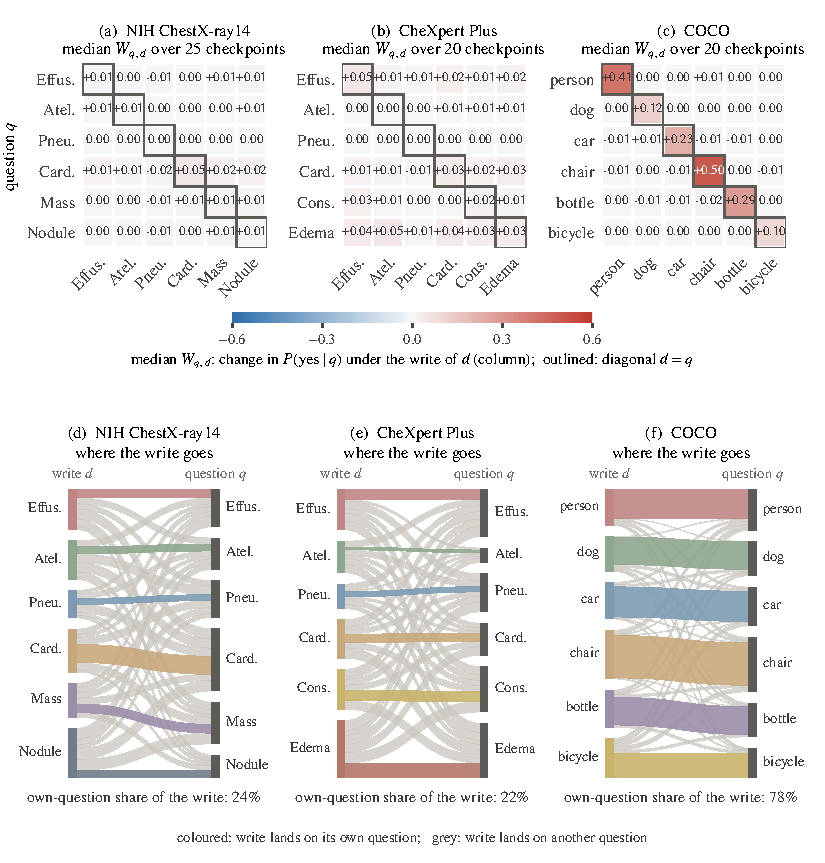
\includegraphics[width=\textwidth]{figures/figA1_write_structure.pdf}
    \caption{\textbf{Write structure across the grid.} (a--c) Cell-wise median of the write matrix $W_{q,d}$ over completed checkpoints on NIH ChestX-ray14, CheXpert Plus, and COCO. (d--f) Where the write goes: bands join each written direction $d$ (left) to the questions $q$ it moves (right), with width proportional to the mean over checkpoints of $\max(W_{q,d},0)$; coloured bands land on the writer's own question, grey bands on another. The share of the write that lands on its own question is printed under each panel.}
    \label{fig:cf-w-structure}
\end{figure}

\subsection{Per-image examples}
\label{app:cf-examples}

Figure~\ref{fig:cf-examples} shows grades on individual test images. For a chest example, the pool contains test rows where the finding is labelled present, the probe reads it (probability above $0.5$), and the clean answer is No. For a natural-image example, the pool contains rows where the probe reads the label correctly and the clean answer is No. We split each pool by whether the concept's own write or the strongest competing write raises the answer more. We show the row whose gap is closest to the median among rows where either write raises the answer by at least $0.2$. Each example's last line reports the number of pool rows with the same ordering, giving that example its own base rate.

\begin{figure}[p]
    \centering
    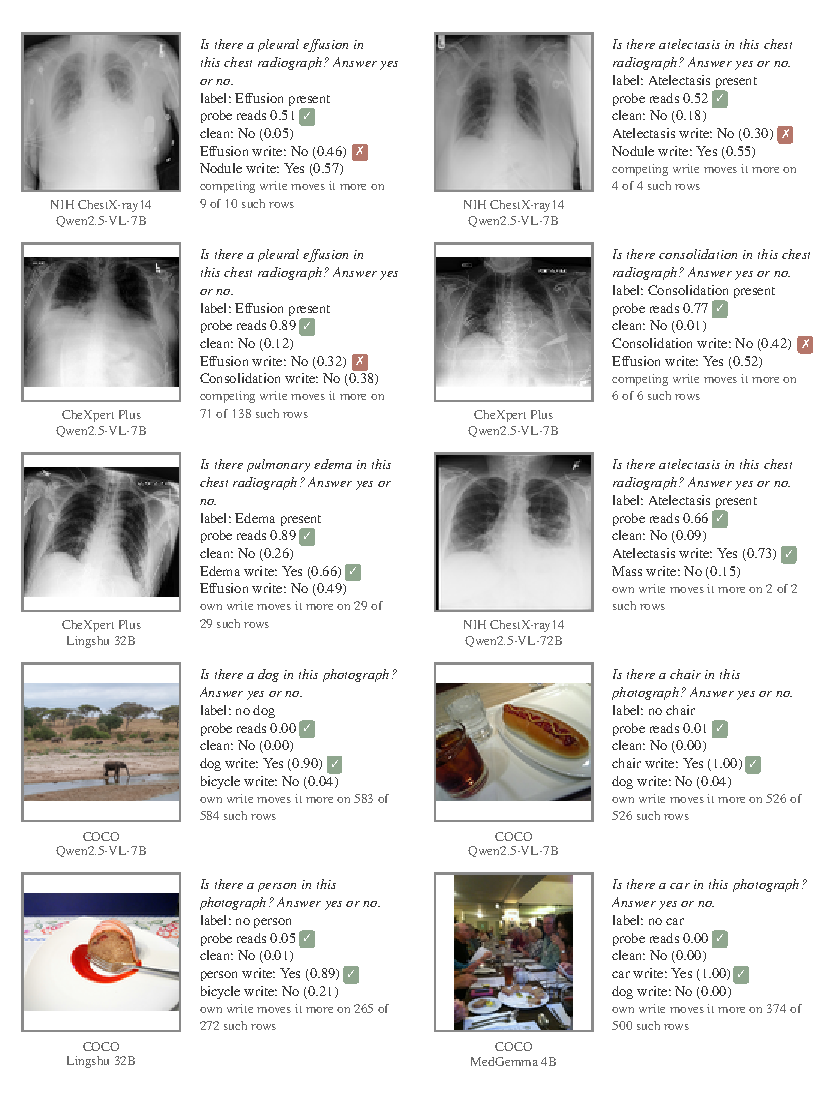
\includegraphics[width=\textwidth]{figures/figA2_examples.pdf}
    \caption{\textbf{Reading, answering, and writing on single images.} For each image: the question, the report label with the probe's reading, the clean answer, the answer under the concept's own write, and the answer under the strongest competing write, all at $\alpha=+0.25$ ($P(\mathrm{yes})$ in parentheses). A check on the write line means the concept's own direction raises its answer more than every competing direction on that image; a cross means a competitor raises it more. The first four chest examples are deficit cells of Qwen2.5-VL-7B; the next two are owned cells (Lingshu 32B Edema, Qwen2.5-VL-72B Atelectasis); the natural-image examples are owned cells of Qwen2.5-VL-7B, Lingshu 32B, and MedGemma 4B. The last line of each example counts the rows of its pool on which the same write wins.}
    \label{fig:cf-examples}
\end{figure}
